% Preamble
% ---
\documentclass[11pt]{article}

% Packages
% ---
\usepackage{amsmath} % Advanced math typesetting
\usepackage[utf8]{inputenc} % Unicode support (Umlauts etc.)
\usepackage[T1]{fontenc}
\usepackage{biolinum}
\usepackage[ngerman]{babel} % Change hyphenation rules
\usepackage[autostyle]{csquotes}
\usepackage{hyperref} % Add a link to your document
\usepackage{graphicx} % Add pictures to your document
\usepackage{listings} % Source code formatting and highlighting
\usepackage{fancyhdr}
\usepackage{biblatex}
\usepackage{pgfplots}
\usepackage{txfonts}
\usepackage{caption}
\usepackage{minted}

\author{Clemens Dautermann}
\title{\Huge Grundbegriffe des maschinellen Lernens\\
	\bigskip
\huge Neuronale Netze \line(1,0){350}
\vspace*{10mm}
\Large Besondere Lernleistung im Fach Informatik
\vspace*{70mm}} 
\date{\today{}}
\pagestyle{fancy}
\captionsetup{justification=raggedright,singlelinecheck=false}

\begin{document}
\biolinum
\pagenumbering{gobble}
\begin{titlepage}
	\maketitle
\end{titlepage}
\pagenumbering{arabic}
\tableofcontents{}
\newpage

\section{Was ist maschinelles Lernen?}
Die wohl bekannteste und am häufigsten zitierte Definiton des maschinellen Lernens stammt von Arthur Samuel aus dem Jahr 1959. Er war Pionier auf diesem Gebiet und rief den Begriff \glqq Machine Learning'' ins Leben. So sagte er:
\begin{quote}
	[Machine learning is the] field of study that gives computers the ability to learn without being explicitly programmed\cite{1}.
	\begin{flushright}
		---Arthur Samuel, 1959
	\end{flushright}
\end{quote}
Beim maschinellen lernen werden Computer also nicht mit einem bestimmten Algorithmus programmiert, um eine Aufgabe zu lösen, sondern lernen eigenständig diese Aufgabe zu bewältigen. Dies geschieht zumeist, indem das Programm aus einer großen, bereits \glqq gelabelten'' Datenmenge mit Hilfe bestimmter Methoden, die im Folgenden weiter erläutert werden sollen, lernt gewisse Muster abzuleiten,  um eine ähnliche Datenmenge selber \glqq labeln'' zu können.  Als Label bezeichent man in diesem Fall die gewünschte Ausgabe des Programms. Dies kann beispielsweise eine Klassifikation sein. Soll das Programm etwa handgeschriebene Ziffern erkennen können, so bezeichnet man das (bearbeitete) Bild der Ziffer als \glqq Input Vector'' und die Information, welche Ziffer der Computer hätte erkennen sollen, als \glqq Label ''. Soll jedoch maschinell erlernt werden, ein simuliertes Auto zu fahren, so bestünde der Input Vector aus Sensorinformationen, und das Label würde aussagen, in welche Richtung das Lenkrad gedreht werden sollte, wie viel Gas das Programm hätte geben sollen oder andere Steuerungsinformationen. Der Input Vector ist also immer die Eingabe, die der Computer erhält um daraus zu lernen, und das Label ist die richtige Antwort, die vom Programm erwartet wurde. Für maschinelles Lernen wird also vor allem eins benötigt: Ein enormer Datensatz, der bereits gelabelt wurde, damit das Programm daraus lernen kann.\newline
Natürlich werden für maschinelles Lernen trotzdem Algorithmen benötigt. Diese Algorithmen sind jedoch keine problemspezifischen Algorithmen, sondern Algorithmen für maschinelles Lernen. Eine der populärsten Methoden des maschinellen Lernens ist das sogenannte \glqq Neuronale Netz''. Dies wird für die zwei Hauptproblemklassen, die man unterscheidet, verwendet: Klassifizierungs und Regressionsprobleme. 
\subsection{Klassifizierungsaufgaben}
Bei einer Klassifizierung werden einer Menge von Eingabevariablen eine diskreten Menge von Ausgabevariablen zugeordnet. Die Ausgabevariablen werden auch als Klassen oder Labels bezeichnet werden. Beispielsweise kann man durch ein Klassifizierungsverfahren eine automatische Spamerkennung bei E-Mails erreichen: Die Eingabevariablen sind die E-Mails und sie sollen den zwei Klassen \glqq Spam'' und \glqq nicht Spam'' zugeordnet werden.\\
Bei dem in dieser Arbeit behandelten Beispiel handelt es sich auch um eine Klassifizierungsaufgabe. Die zu klassifizierenden Bilder von Ziffern sollen den zehn Klassen \glqq 0'' bis \glqq 9'' zugeordnet werden. Die Bilder sind hier die Eingabevariablen und die Klassen \glqq0'' bis \glqq9'' beschreibt die endliche Menge diskreter Labels.\\
Das erste Beispiel, bezogen auf die Spam-Mails, würde man als \glqq Binärklassifizierung'' bezeichnen, da zwei Klassen unterschieden werden. Letzteres wird als \glqq Multiklassenklassifizierung'' bezeichnet, da mehr als zwei Klassen unterschieden werden. Die Binärklassifizierung ist in Abbildung \ref{Classification} verdeutlicht.
\begin{figure}[h]
	\centering
	\includegraphics[width=0.5\linewidth]{../graphics/Classification.png}
	\caption{Die zwei Klassen wären hier \glqq grün'' und \glqq blau''. Die Linie stellt die Klassengrenze dar, die die zwei Klassen unterscheidet. Es sind außerdem einige Ausreißer in den Daten vorhanden. }
	\label{Classification}
\end{figure}
\subsection{Regressionsprobleme}
Als Regressionsproblem hingegen bezeichnet man das Finden einer Funktion, die eine Menge von Eingabevariablen einer stetigen Menge von Ausgabevariablen zuordnet. Wenn beispielsweise ein Bild eines Menschen gegeben ist, könnte ein Regressionsproblem sein, seine Höhe oder sein Gewicht zu bestimmen. Auch eine Wettervorhersage ist ein typisches Regressionsproblem. Ein Beispiel eines Regressionsproblemens wird in dieser Arbeit nicht behandelt werden. Wie Regression dargestellt werden kann, ist in Abbildung \ref{Regression} gezeigt.
\begin{figure}[h]
	\centering
	\includegraphics[width=0.5\linewidth]{../graphics/Regression.png}
	\caption{Die Kurve stellt hier keine Grenze, sondern die Funktion, die die Werte approximiert, dar. Die Punkte repräsentieren die Eingabedaten, wobei auch hier einige Ausreißer erkennbar sind.}
	\label{Regression}
\end{figure}
\\
Regression wird daher auch als \glqq Curve-Fitting'' bezeichnet. Eine Kurve soll also bestmöglich eine Datenmenge approximieren, und eine Vorhersage an Stellen wo keine Daten vorhanden sind treffen.
\subsection{Gefahren von maschinellem Lernen}
Maschinelles Lernen kann eine mächtige Technologie sein. Eine Vielzahl von Problemen lässt sich damit lösen, alle jedoch nicht. Bevor man maschinelles Lernen nutzt, sollte man sich also fragen: Lässt sich dieses Problem nicht einfacher auf konventionelle Weise lösen? Zu den prinzipiellen Schwierigkeiten von maschinellem Lernen gehört, dass es unter ungünstigen Umständen fehleranfällig sein kann und deswegen am besten mit anderen Verfahren kombiniert werden sollte. In Systemen, wo eine korrekte Antwort kritisch ist, sollte man also nicht alleine auf maschinelles Lernen setzen.\\
Auch ist für maschinelles Lernen stets eine enorme Datenmenge nötig. Diese Daten müssen erst gesammelt werden. Hier stellt sich natürlich sofort eine ethische Frage: Welche Daten können guten Gewissens gesammelt und ausgewertet werden? Dabei sollten das Persönlichkeitsrecht und das Recht auf Privatsphäre eine zentrale Rolle spielen. Niemals sollte der Nutzen der Technologie über die Rechte der Nutzer gestellt werden. Betrachtet man hier beispielsweise den Flughafen von Peking, sind erschreckende Tendenzen festzustellen. Dort wird beim Check-In via Gesichtserkennung die Identität der Person mit ihrem Gesicht verknüpft. Danach läuft alles vom Ticketkauf bis hin zum Duty-free-shop mit Hilfe von Gesichtserkennung ab \cite{4}.\\
Die zentralen Gefahren maschinellen Lernens sind also die eventuelle Unsicherheit im Ergebnis, der hohe Trainingsaufwand, der gegebenenfalls mit klassischen Algorithmen vermieden werden kann, und die Verletzung von Rechten durch das Auswerten persönlicher Daten.

\subsubsection{Datensätze für maschinelles Lernen}
Wie bereits erwähnt, sind die Datensätze oft der limitierende Faktor beim maschinellen Lernen. Das gravierendste Problem ist, überhaupt einen passenden Datensatz für das Problem zu finden oder generieren zu können: Dabei muss man beachten, dass man alle für das Problem relevanten Faktoren berücksichtigt. Möchte man beispielsweise Gesichter jeglicher Art erkennen, genügt es nicht den Algorithmus auf einem Datensatz von Gesichtern hellhäutiger Menschen zu trainieren, da dieser zum Erkennen von Gesichtern dunkelhäutiger Menschen nutzlos wäre. Dass dies kein theoretisches, sondern auch ein praktisch auftretendes Phänomen ist, zeigt eine Studie des National Institute for Standards and Technology (NIST)\cite{5}. Diese hat ergeben, dass beispielsweise ein in den USA entwickelter und dort sehr populärer Algorithmus eine extrem hohe Fehlerquote für afroamerikanische Frauen hat. Da dieses System unter anderem von der Polizei in den USA verwendet wird, haben afroamerikanische Frauen eine wesentlich höhere Chance, fälschlicherweise einer Straftat beschuldigt zu werden als andere Bürger.\\
Man sollte außerdem beachten, dass der Datensatz gut ausgeglichen ist. Das bedeutet, dass alle Trainingsdaten gleichmäßig verteilt sind. Möchte man beispielsweise Eingabedaten in 4 verschiedene Klassen klassifizieren, so sollten etwa 25\% der Daten zur Klasse A gehören, 25\% zur Klasse B und so weiter. Der in dieser Arbeit später verwendete MNIST Datensatz hat einen Umfang von 60000 handgeschriebenen Ziffern von 0 bis 9. Den größten Anteil haben Einsen mit rund 11\%, den niedrigsten haben Fünfen mir 9\%. Damit kann der Datensatz als ausgeglichen betrachtet werden. Eine genaue Definition, ab wann ein Datensatz nicht mehr ausgeglichen ist, existiert nicht.\\
Datensätze müssen ausgeglichen sein, da das Netz sonst den Fehler, der im Folgenden noch erläutert werden wird, minimiert, indem es öfter die Klasse mit dem höchsten Anteil als Antwort liefert. Es erkennt, dass die höchste Trefferquote vorliegt, wenn es diese Antwort gibt, da so die Wahrscheinlichkeit eines Treffers maximal ist\footnote{In diesem Fall wird dann in der Fehlerfunktion ein lokales Minimum gefunden. Dazu mehr unter Abschnitt \ref{Gradient_section}, \nameref{Gradient_section}}.
\subsubsection{Overfitting}
Overfitting ist ein häufig auftretendes Problem bei Klassifizierungsaufgaben. Die Klassengrenzen werden dabei zu sehr an die Trainingsdaten angepasst und dadurch falsch definiert. In Abbildung \ref{Overfitting} ist dies dargestellt.
\begin{figure}[h]
	\centering
	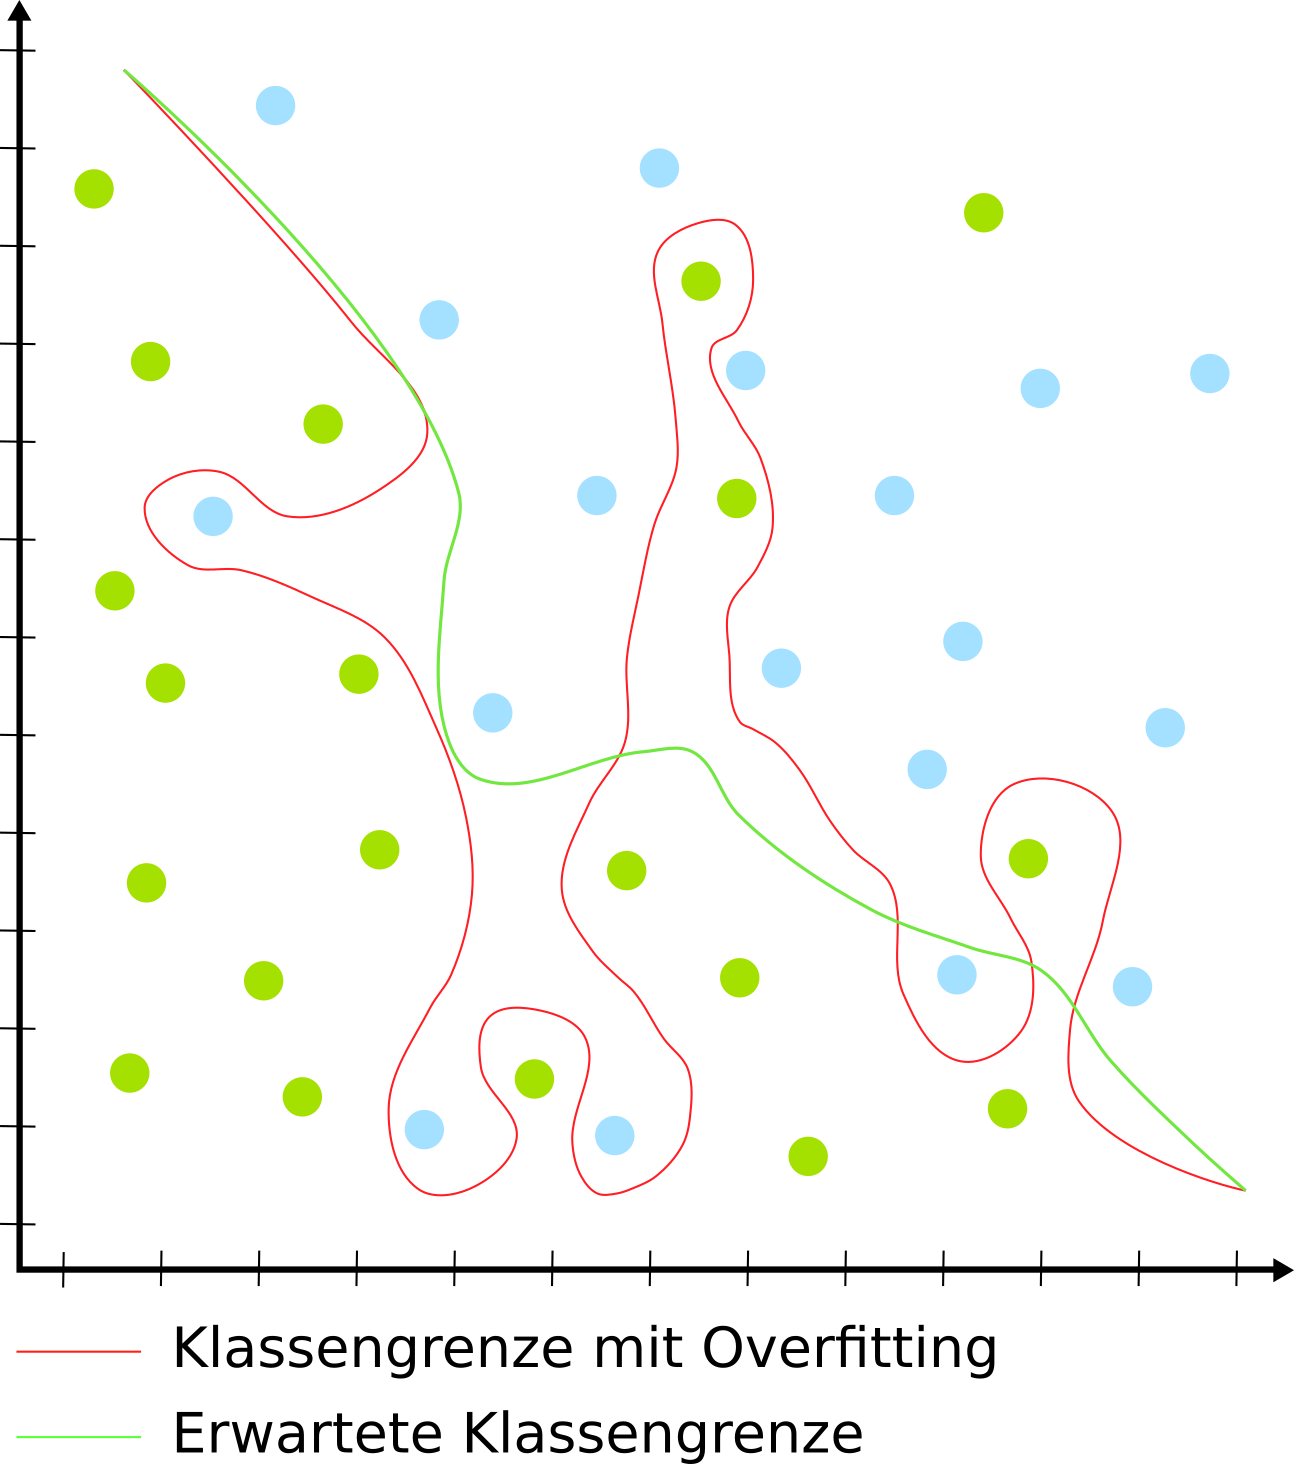
\includegraphics[width=0.5\linewidth]{../graphics/overfitting.png}
	\caption{Klassengrenzen mit und ohne Overfitting}
	\label{Overfitting}
\end{figure}
\\
Overfitting tritt auf, wenn man ein neuronales Netz zu lange auf einem Datensatz trainiert. Das Netz lernt dann die Daten auswendig, da es so einen Fehler von 0 erreichen kann. Dadurch werden aber keine wirklichen Klassengrenzen erlernt.\\
Um Overfitting entgegenzuwirken, reicht es oftmals, den Trainingsdatensatz in der Reihenfolge zu randomisieren. Dadurch kann das Netz die Reihenfolge gar nicht auswendig lernen.
\subsection{Adversarial attacks}
Sogenannte \glqq Adversarial attacks'' können genutzt werden, um neuronale Netze gezielt zu täuschen. Dabei werden die Eingabedaten so manipuliert, dass für einen Menschen kaum ein Unterschied erkennbar ist, das neuronale Netz sie jedoch falsch klassifiziert. Dafür wird meist ein anderes neuronales Netz genutzt, das innerhalb eines gewissen Maßes die Daten verändert. Der Änderungsspielraum wird dabei so festgelegt, dass ein Mensch keinen Unterschied wahrnehmen kann. Dieses Netz versucht dann, eine Ausgabe zu erzeugen, sodass der Unterschied minimal und der Fehler des Klassifizierungsnetzwerkes maximal wird. So werden die Daten möglichst falsch klassifiziert, und der Unterschied ist trotzdem nicht erkennbar. Dies gelingt besonders gut bei Bildern, ist jedoch auch auf Text übertragbar, wie Di Jin, Zhijing Jin, Joey Tianyi Zhou und Peter Szolovits 2019 gezeigt haben\cite{8}. Die Gefahr bei Adversarial Attacks besteht darin, dass eine beliebige Ausgabe erzeugt werden kann. Es ist also nicht nur möglich, einen Fehler zu erzeugen, sondern dieser ist auch noch genau steuerbar. Dabei kann die Genauigkeit bekannter Bildklassifizierungsnetzwerke erheblich gesenkt werden\cite{9}. 
\section{Verschiedene Techniken maschinellen Lernens}\label{sec:verschiedene-techniken-maschinellen-lernens}
Es gibt viele verschiedene Ansätze und Algorithmen, um maschinelles Lernen zu implementieren. Der wohl häufigste ist das Neuronale Netz, von dem diese Arbeit handelt. Aber auch sogenannte \glqq Support Vector machines'' sind eine bekannte Technik, sollen aber hier nicht weiter behandelt werden. Neuronale Netze können in vielen verschiedenen Szenarien angewandt werden, um unterschiedliche Ergebnisse zu erzielen. Beim Adversarial Learning lässt man mehrere Netze gegeneinander antreten, sodass sie sich gegenseitig trainieren. Beim Q-Learning beginnt man mit zufälligen Reaktionen auf eine Eingabe und \glqq belohnt'' das Netz, falls es wie gewünscht reagiert hat. Ein Beispiel hierfür ist die \glqq Hide and Seek AI'' von OpenAI\footnote{https://openai.com/blog/emergent-tool-use/}. Grob unterscheidet man jedoch in überwachtes (supervised), unüberwachtes (unsupervised) und bestärkendes (reinforced) Lernen.
\subsection{Überwachtes Lernen}
Beim Überwachten Lernen ist ein Trainingsdatensatz vorhanden und, die Eingabe sowie die gewünschte Ausgabe sind bekannt. Dies trifft sowohl auf Klassifizier\-ungs- als auch auf Regressionsprobleme zu. Um überwachtes Lernen nutzen zu können, muss man also vor allem über einen großen Datensatz verfügen. Wie genau Überwachtes Lernen innerhalb des neuronalen Netzes vonstatten geht, ist im nächsten Abschnitt unter \glqq\nameref{sec:neuronale-netze}'' beschrieben.
\subsection{Unüberwachtes Lernen}
Unüberwachtes Lernen erkennt automatisiert Muster in Datenmengen. Dies ist vergleichbar mit einem Kind, das zum ersten Mal in seinem Leben einen Hund sieht und den nächsten Hund, den es sieht, als solchen wiedererkennt. Das Kind hat nicht, wie es beim überwachten Lernen der Fall gewesen wäre, gesagt bekommen, dass es sich um einen Hund handelt. Vielmehr hat es die Merkmale eines Hundes erkannt und sich diese gemerkt.
Bei unüberwachtem Lernen werden also automatisch Muster erkannt, die dem Algorithmus zuvor nicht mitgeteilt wurden. 
\subsection{Bestärkendes Lernen}
Bestärkendes Lernen ist der letzte der drei häufig unterschiedenen Lerntypen. Hier ist kein Eingabedatensatz vorhanden, sondern ein bekanntes Ziel definiert. Der Algorithmus soll einen möglichst effizienten Weg finden, dieses Ziel zu erreichen. Oft ist dabei ein Handlungsträger (Agent) in einer Umgebung gegeben. Dies kann beispielsweise ein Auto sein, das lernen soll selbst zu fahren. Auch die in Abschnitt  \ref{sec:verschiedene-techniken-maschinellen-lernens} erwähnte Q-Learning Methode aus open-AIs \glqq hide and seek AI'' fällt in die Kategorie des bestärkenden Lernens. Der durch die KI gesteuerte Handlungsträger beginnt mit zufälligen Handlungen und erhält, wenn er ein Zwischenziel erreicht, Belohnungen oder Strafen, wenn er einen Fehler macht. Diese Belohnungen und Strafen werden in Form von Zahlen vergeben. Das selbstfahrende Auto würde beispielsweise eine Belohnung erhalten, wenn es einen Streckenabschnitt fehlerfrei zurückgelegt hat, und eine Strafe, wenn es gegen eine Wand fährt. Das Ziel ist es, diese kumulativen Belohnungen zu maximieren und dadurch das vordefinierte Ziel zu erreichen. Hierfür häufig verwendete Algorithmen sind das Q-learning oder sogenannte \glqq Monte-Carlo Maschinen''.
\section{Neuronale Netze}\label{sec:neuronale-netze}
Bei Neuronalen Netzen handelt es sich um eine programminterne Struktur, die für das maschinelle Lernen genutzt wird. Wie der Name bereits vermuten lässt, ist diese Methode ein Versuch, das menschliche Lernen nachzuahmen.
\subsection{Maschinelles Lernen und menschliches Lernen}
Das menschliche Gehirn ist aus sogenannten \glqq Neuronen'' aufgebaut. Ein Neuron ist eine Nervenzelle, die elektrische oder chemische Impulse annimmt und gegebenenfalls einen elektrischen oder chemischen Impuls weitergibt. Die Nervenzellen berühren sich nicht direkt, sondern sind nur über die sogenannten Synapsen verbunden, über die diese Signale übertragen werden, sodass sich ein hoch komplexes Netzwerk von Milliarden von Neuronen ergibt.\footnote{
Diese Definition ist stark vereinfacht. Sie enthält ausschließlich die wesentlichen Komponenten, um das menschliche Gehirn mit einem neuronalen Netz vergleichen zu können.}
\begin{figure}[h]
	\centering
	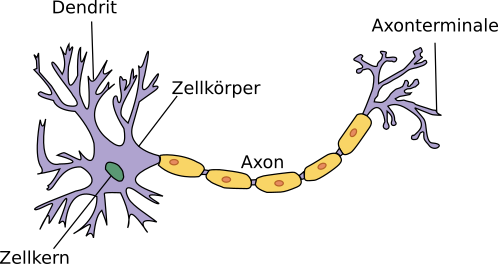
\includegraphics[]{../graphics/Neuron.png}
	\caption[Neuron \newline 
	Quelle: simple.wikipedia.org/wiki/File:Neuron.svg\newline
	Copyright: CC Attribution-Share Alike von Nutzer Dhp1080,\newline
 	bearbeitet]{Vergleichende Darstellung eines Neurons im menschlichen Gehirn}
\end{figure}
Ein neuronales Netz ist ähnlich aufgebaut. Es besteht aus \glqq Neuronen'', die eine theoretisch beliebige Anzahl von Eingaben annehmen können und mit einer entsprechenden Ausgabe reagieren, sowie Verbindungen zwischen den Neuronen. Auch das Lernprinzip entspricht dem eines Menschen. Das Netz nimmt meist Zahlen zwischen 0 und 1 als Eingabe an und berechnet eine entsprechende Ausgabe. Es erhält anschließend die Information, wie die richtige Lösung gelautet hätte und lernt dann aus seinen Fehlern, indem es gewisse Werte, die in die Berechnung einfließen, anpasst. Analog lernt ein Mensch, indem er ausprobiert, gegebenenfalls scheitert, anschließend die richtige Antwort durch eine externe Quelle erhält und somit aus seinem Fehler lernt. Im menschlichen Gehirn verknüpfen sich dabei oft genutzte neuronale Verbindungen stärker und weniger benutzte Verbindungen bauen sich ab\cite{2}. Die Verstärkung und der Abbau entsprechen der Änderung der Gewichtung einer Verbindung im neuronalen Netz. Die Gewichtung ist eine Eigenschaft der Verbindung, die eine zentrale Rolle in der Berechnung spielt, und soll im folgenden weiter erläutert werden. Diese Ähnlichkeiten zwischen maschinellem und menschlichem Lernen sind kein Zufall, sondern viel mehr Intention. Ein neuronales Netz ist nämlich der gezielte Versuch das menschliche Lernen nachzuahmen, um maschinelles Lernen zu ermöglichen.
\subsection{Der Aufbau eines neuronalen Netzes}
Ein neuronales Netz besteht aus Neuronen und Verbindungen zwischen diesen. Eine Schicht von Neuronen wird auch als Layer bezeichnet und die Verbindungen als Kanten. Es gibt einen sogenannten \glqq Input Layer'', der die Daten (also meist die Zahlen von 0 bis 1), den sogenannten \glqq Input Vector'', annimmt, eine beliebige Anzahl von sogenannten \glqq Hidden Layers'', in denen das eigentliche Lernen statt findet, und einen sogenannten \glqq Output Layer'', der für die Datenausgabe verantwortlich ist. Die Anzahl der Neuronen ist nach oben nicht begrenzt, wird jedoch zumeist der Aufgabe angepasst. Im Input Layer ist meist ein Neuron pro Pixel des Eingabebildes vorhanden und im Output Layer ein Neuron pro möglicher Ausgabe. Sollen also 28$\times$28 Pixel große Bilder handgeschriebener Ziffern klassifiziert werden, so gibt es 784 Eingabeneuronen, da jedes Bild 784 Pixel groß ist\footnote{Bilder sind als Matrizen gespeichert. Um sie in das Netz einlesen zu können, müssen sie erst in einen Vektor konvertiert werden. Diesen Vorgang beschreibt man als \glqq flattening''}, und 10 Ausgabeneuronen, da es 10 Ziffern gibt.
\begin{figure}[h]
\centering
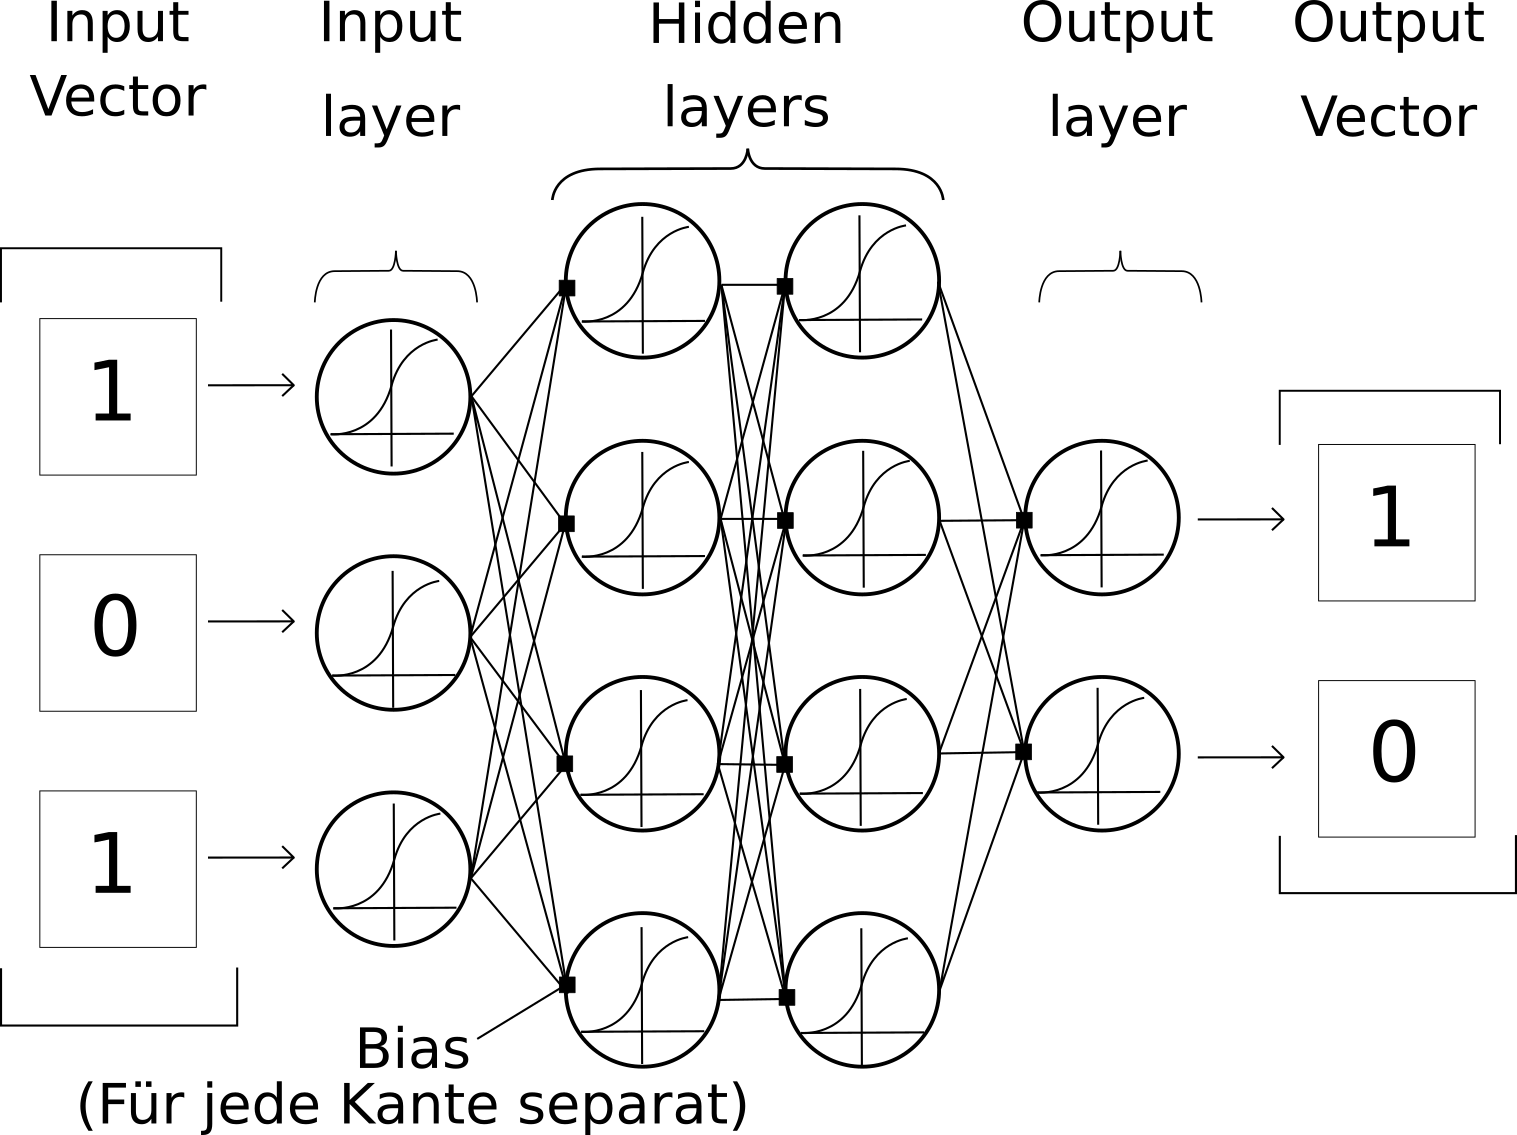
\includegraphics[width=\linewidth]{../graphics/Neural_Net.png}
\caption{Schematische Darstellung eines einfachen neuronalen Netzes}
\end{figure}
Jedes Neuron hat außerdem eine sogenannte Aktivierungsfunktion, die sich von Neuron zu Neuron unterscheiden kann, und jede Kante eine asoziierte Gewichtung und einen Bias. Ein neuronales Netz besteht also aus:
\begin{itemize}
	\item Neuronen mit gegebenenfalls verschiedenen Aktivierungsfunktionen, aufgeteilt in ein Input-, beliebig viele Hidden- und ein Output-Layer.
	\item Verbindungen zwischen diesen Neuronen, die jeweils einen eigenen Bias und eine Gewichtung besitzen, und als Kanten bezeichnet werden.
\end{itemize}
Sind alle Neuronen eines Layers jeweils mit allen Neuronen des nächsten Layers verbunden, wird das Layer als \glqq Fully Connected Layer'' bezeichnet.
\subsection{Berechnung des Ausgabevektors}
Der Ausgabevektor wird berechnet, indem:
\begin{enumerate}
	\item Alle Ausgaben aus der vorherigen Schicht mit der Gewichtung der korrespondierenden Kante multipliziert werden.
	\item Alle gewichteten Eingabewerte summiert werden.
	\item Der Bias des Neurons hinzu addiert wird.
	\item Die Aktivierungsfunktion auf diesen Wert angewandt wird.
\end{enumerate}
Die Aktivierungsfunktion soll dabei die Werte zu normieren. Sie sorgt also dafür, dass alle Werte innerhalb des Netzes im Intervall $[0, 1]$ bleiben. Es gibt eine Vielzahl von Aktivierungsfunktionen. Die häufigste ist die in Abbildung \ref{Sigmoid} dargestellte \glqq Sigmoid'' Funktion. Aber auch die in Kapitel \ref{sec:das-netz} näher erläuterte \glqq ReLu'' Funktion ist recht populär.
\begin{figure}[h]
\begin{center}
\begin{tikzpicture}
	\begin{axis}[samples=100, width=0.5\linewidth]
		\addplot[blue]{tanh(x)};
	\end{axis}
\end{tikzpicture}
\end{center}
\caption{Darstellung der Sigmoid-Funktion $\sigma(x)=\frac{e^x}{e^x+1}$ im Intervall $[-5, 5]$}
\label{Sigmoid}
\end{figure}
\\
Im Gegensatz dazu haben Gewichtungen typischerweise etwa den doppelten Wert der Eingaben. Alle Werte werden jedoch automatisch im Lernprozess angepasst.
\\
Die Begriffe Eingabe- und Ausgabevektor lassen bereits vermuten, dass es sich bei Neuronalen Netzen um Objekte aus dem Bereich der linearen Algebra handelt. Daher wird im Folgenden auch die Notationsweise mit Hilfe von linearer Algebra verwendet. Betrachtet man eine Ausgabe eines Neurons, wird diese als $a^ {layer}_{neuron}$ bezeichnet. Den Ausgabevektor des Input Layers würde man also folgendermaßen schreiben:
\begin{equation*}
\begin{bmatrix}
	a^0_0\\
	a^0_1\\
	a^0_2\\
	\vdots\\
	a^0_n
\end{bmatrix}
\end{equation*}
Die Gewichtungen $w$ der jeweiligen Kanten werden als $w^{(von\ Layer)}_{(zu\ Neuron,\ von\ Neuron)}$ notiert. \glqq Von Layer'' bezeichnet dabei das Layer, in dem das Neuron liegt, das die Information ausgibt. \glqq Zu Neuron'' ist der Index des Neurons im nächsten Layer, das die Information annimmt und \glqq von Neuron'' der Index des Neurons, das die Information abgibt. Die Gewichtung der Kante, die das zweite Neuron im ersten Layer mit dem dritten Neuron im zweiten Layer verbindet, würde also als $w^0_{3,2}$ bezeichnet werden. Dabei wird bei Null begonnen zu zählen, sodass das erste Layer und das erste Neuron jeweils den Index 0 erhält.\newline
Die Gewichtungen aller Verbindungen eines Layers zum nächsten können also als folgende Matrix geschrieben werden:
\begin{equation*}
	\begin{bmatrix}
	w_{0,0} & w_{0,1} & \cdots & w_{0,n}\\
	w_{1,0} & w_{1,1} & \cdots & w_{1,n}\\
	\vdots & \vdots & \ddots & \vdots\\
	w_{k,0} & w_{k,1} & \cdots & w_{k,n}\\
	\end{bmatrix}
\end{equation*}
Dabei ist $n$ hier dieselbe Zahl wie $n$ im Ausgabevektor, da genau so viele Ausgaben vorhanden sein müssen, wie Neuronen in diesem Layer vorhanden sind, da jedes Neuron einen Wert ausgibt\footnote{Es existieren auch Neuronen, die Daten verwerfen. Diese kommen im hier betrachteten Typ von neuronalem Netz allerdings nicht vor und werden daher der Einfachheit halber außenvor gelassen.}. Der Bias Vektor wird genau so wie der Ausgabevektor bezeichnet:
\begin{equation*}
\begin{bmatrix}
	b^0_0\\
	b^0_1\\
	b^0_2\\
	\vdots\\
	b^0_n
\end{bmatrix}
\end{equation*}
\newpage
Beachtet man jetzt noch, dass bei jedem Neuron die Aktivierungsfunktion angewandt werden muss, ergibt sich folgende Gleichung für die Berechnung des Ausgabevektors $\vec{o}$ aus einem Einbagevektor $\vec{a}$ durch eine Schicht von Neuronen:
\begin{figure}[h]
	\begin{equation*}
		\vec{o} = \sigma\left(
		\begin{bmatrix}
			w_{0,0} & w_{0,1} & \cdots & w_{0,n}\\
			w_{1,0} & w_{1,1} & \cdots & w_{1,n}\\
			\vdots & \vdots & \ddots & \vdots\\
			w_{k,0} & w_{k,1} & \cdots & w_{k,n}\\
		\end{bmatrix}
		\begin{bmatrix}
			a^0_0\\
			a^0_1\\
			a^0_2\\
			\vdots\\
			a^0_n
		\end{bmatrix}
		+
		\begin{bmatrix}
			b^0_0\\
			b^0_1\\
			b^0_2\\
			\vdots\\
			b^0_n
		\end{bmatrix}
		\right)
	\end{equation*}
	\caption{Formel zur Berechnung eines Ausgabevektors aus einem Eingabevektor durch eine Schicht von Neuronen. }
\end{figure}
\newline
Zur Vereinfachung wurde die Funktion hier auf den gesamten Ausgabevektor angewandt. Dies ist korrekt, sofern alle Neuronen eines Layers dieselbe Aktivierungsfunktion aufweisen. Dies muss natürlich nicht immer so sein. Sind die Aktivierungsfunktionen der Neuronen eines Layers verschieden, so wird die Aktivierungsfunktion des jeweiligen Neurons separat auf das korrespondierende Element des Vektors $W\cdot\vec{a}+\vec{b}$ angewandt.
\subsection{Der Lernprozess}
Der Lernprozess gliedert sich in wenige wesentliche Schritte. Zuerst wird unter Verwendung des oben beschriebenen Prozesses aus einem Eingabevektor ein Ausgabevektor berechnet. Diese Berechnung wird im Lernprozess extrem oft durchgeführt, weshalb sich neuronale Netze besonders schnell auf Grafikkarten trainieren lassen, da diese für mathematische Operationen im Bereich der linearen Algebra wie Matritzenmultiplikation oder -Addition optimiert sind, indem sie dafür erforderliche Operationen sehr schnell und teilweise auch parallel (Vektorprozessierung) ausführen können.\\
Dieser Ausgabevektor wird nun, mit Hilfe einer Fehlerfunktion, mit dem erwarteten Ausgabevektor verglichen. Je größer dabei die Differenz zwischen erwartetem Ausgabevektor und tatsächlichem Ausgabevektor ist, desto größer ist der Wert der Fehlerfunktion. Der Ausgabewert dieser Fehlerfunktion wird als \glqq Fehler'' oder auch als \glqq Kosten'' bezeichnet. Wenn also das Minimum dieser Fehlerfunktion bestimmt wird, wird der Fehler minimiert, und die tatsächliche Ausgabe des Netzes nähert sich der korrekten Ausgabe immer weiter an.\newline
Eine Methode dieses Minimum zu finden, ist das Gradientenverfahren. Nachdem mit Hilfe dieses Verfahrens der Fehler mimimiert wurde, werden die Parameter, also die Gewichtungen und Biases\footnote{Es gibt Netzarten, die mehr anpassbare Parameter aufweisen.}, des neuronalen Netzes entsprechend angepasst. Diesen Prozess der Fehlerminimierung mittels des Gradientenverfahrens und der anschließenden Anpassung der Werte bezeichnet man auch als \glqq Backpropagation''. Es existieren auch noch andere Verfahren zur Fehlerminimierung, der Einfachheit halber soll hier aber nur Backpropagation erläutert werden.
\subsection{Fehlerfunktionen}
Es existiert eine Vielzahl von Fehlerfunktionen, die alle für unterschiedliche Anwendungsgebiete passend sind. Im Groben lassen sich allerdings Fehlerfunktionen, die für Klassifizierungsprobleme geeignet sind, von solchen unterscheiden, die für Regressionsprobleme geeignet sind.
\subsubsection{MSE -- Durchschnittlicher quadratischer Fehler}
Der sogenannte durchschnittliche quadratische Fehler ist eine häufig genutzte Fehlerfunktion für Regressionsprobleme, die nicht nur für Regression im Bereich des maschinellen Lernens verwendung findet, sondern auch bei statistischer Regression populär ist. Die englische Bezeichnung lautet \glqq Mean squared error'', woraus sich auch die Abkürzung \glqq MSE loss'' ergibt. Sie ist wie in Abbildung \ref{MSE_equation} dargestellt, definiert.
\begin{figure}[h]
	\begin{equation*}
		\textrm{MSE}=\dfrac{\sum\limits_{i=1}^n(y_i-\hat{y_i})^2}{n}
	\end{equation*}
	\caption{Die Gleichung für den durchschnittlichen quadratischen Fehler}
	\label{MSE_equation}
\end{figure}
\newline
Wie der Name vermuten lässt, gibt diese Fehlerfunktion den Durchschnitt der quadrierten Differenzen zwischen dem vorausgesagten und dem tatsächlichen Ergebnis an. Aufgrund der Quadrierung des Fehlers werden durch diese Funktion stark abweichende Werte wesentlich stärker gewichtet, als weniger abweichende Werte. Ihr Gradient ist außerdem einfach berechenbar, was für das Gradientenverfahren später relevant ist.\cite{3}
\subsubsection{MAE -- Durchschnittlicher absoluter Fehler}
Bei dem durchschnittlichen absoluten Fehler handelt es sich ebenfalls um eine Fehlerfunktion, die für Regressionsprobleme eingesetzt wird. Die englische Bezeichnung lautet \glqq Mean absolute error''. Sie ist ähnlich wie der durchschnittliche quadratische Fehler definiert.
\begin{figure}[h]
	\begin{equation*}
	\textrm{MAE}=\dfrac{\sum\limits_{i=1}^n|y_i-\hat{y_i}|}{n}
	\end{equation*}
	\caption{Die Gleichung für den durchschnittlichen absoluten Fehler}
	\label{MAE_equation}
\end{figure}
\newline
Auch hier wird die \glqq Richtung'' des Fehlers, in diesem Fall durch die Normierung, verworfen. Außerdem ist diese Fehlerfunktion nicht so anfällig gegenüber Ausreißern in den Daten, da dieser Fehler nicht quadriert wird. Ein Nachteil des durchschnittlichen absoluten Fehlers ist allerdings die höhere Komplexität zur Berechnung des Gradienten.\cite{3}
\subsubsection{Kreuzentropiefehler}
Der Kreuzentropiefehler ist die am häufigsten verwendete Fehlerfunktion für Klassifizierungsprobleme. Sie gibt den Fehler für eine Klassifizierung an, die den gegebenen Klassen Wahrscheinlichkeiten im Intervall $I=[0;1]$ zuordnet. Dabei steigt der Fehler stärker, je weiter sich die Vorhersage vom tatsächlichen Wert entfernt. Wie aus Abbildung \ref{CEL_Graph} hervorgeht, wird also sicheren, aber falschen Vorhersagen der höchste Fehlerwert zugeordnet. 
\begin{figure}[h]
	\begin{center}
		\begin{tikzpicture}
		\begin{axis}[width=0.60\linewidth, 
		xmax=1, 
		ymax=10, 
		xmin=0, 
		samples=10000,
		xlabel={vorhergesagte Wahrscheinlichkeit},
		ylabel={Kreuzentropiefehler}]
		\addplot[blue]{-ln(x))};
		\end{axis}
		\end{tikzpicture}
	\end{center}
	\caption{Der Graph der Kreuzentropie-Fehlerfunktion, wenn das tatsächliche Label 1 ist}
	\label{CEL_Graph}
\end{figure}
\\
Der Fehler steigt also mit zunehmender Abweichung der Vorhersage zum tatsächlichen Label rapide an.\newline 
Mathematisch ist der Kreuzentropiefehler nach der Funktion in Abbildung \ref{CEL_Function} definiert, wobei $y$ einen Binärindikator darstellt, der angibt, ob das zu klassifizierende Objekt tatsächlich zur Klasse gehört (dann ist er 1), und $p$ die vorausgesagte Wahrscheinlichkeit, ob das Objekt zur Klasse gehört, beschreibt.
\begin{figure}[h]
	\begin{equation*}
	\textrm{CrossEntropyLoss}=-(y\ln(p)+(1-y)\ln(1-p))
	\end{equation*}
	\caption{Die Gleichung für den Kreuzentropiefehler}
	\label{CEL_Function}
\end{figure}
\newline
Hier fällt auf, dass, falls das Label 0 ist, der linke Teil der Gleichung wegfällt, und falls es 1 ist, der rechte. Wenn berechnetes und tatsächliches Label identisch sind, ist der Fehler stets 0.\\
Existieren mehr als 2 Klassen, handelt es sich also nicht mehr um eine Binärklassifizierung müssen die Fehler nach der Gleichung in Abbildung \ref{CEL_Function_cummulative} summiert werden.
\begin{figure}[h]
	\begin{equation*}
	\textrm{CrossEntropyLoss(M)}=-\sum\limits_{c=1}^My_{o,c}ln(p_{o,c})
	\end{equation*}
	\caption{Die Gleichung für den durchschnittlichen absoluten Fehler}
	\label{CEL_Function_cummulative}
\end{figure}
\newline
Dabei gibt $M$ die Anzahl der Klassen an, $c$ das Label für die Klasse und $o$ die berechnete Klassifizierung für diese Klasse.
\subsection{Gradientenverfahren und Backpropagation}
\label{Gradient_section}
Das Gradientenverfahren ist ein Verfahren, um das Minimum einer Funktion zu finden. Die Funktion, deren Minimum gefunden werden soll, ist in diesem Fall die Fehlerfunktion. Diese ist von allen Gewichtungen und Biases des Netzwerkes abhängig, da sie direkt vom Ausgabevektor des Netzes abhängig ist. Der Gradient dieser Funktion ist in Abbildung \ref{Gradient_Function} dargestellt.
\newpage
\begin{figure}[h]
	\begin{equation*}
	\nabla C(w_1,b_1,\ldots,w_n,b_n)=
	\begin{bmatrix}
		\frac{\partial C}{\partial w_1}\\
		\frac{\partial C}{\partial b_1}\\
		\vdots\\
		\frac{\partial C}{\partial w_n}\\
		\frac{\partial C}{\partial b_n}
	\end{bmatrix}
	\end{equation*}
	\caption{Die Gleichung für den Gradienten der Fehlerfunktion}
	\label{Gradient_Function}
\end{figure}
Um also das Ergebnis \glqq richtiger'' zu machen, müssen alle Gewichtungen und Biases negativ zu diesem Gradienten angepasst werden, da der Gradient ja in Richtung Hochpunkt zeigt. Diese Anpassung erfolgt, indem das Netz vom Ausgabelayer an rückwärts durchgegangen wird, und die Gewichtungen und Biases angepasst werden. Deshalb heißt das Verfahren Backpropagation.\\
Oft wird zur Verbildlichung des Gradientenverfahrens die Analogie eines Balles verwendet, der einen Hügel hinunter rollt. Er findet den Tiefpunkt, indem er hinab rollt. Dabei wirkt immer automatisch eine Kraft nach unten.
\subsubsection{Lernrate}
Eine wichtige Rolle dabei spielt die sogenannte \glqq Lernrate'' $\eta$, mit der die Änderung nach der Formel in Abbildung \ref{Learning_Rate_Function} berechnet wird.
\begin{figure}[h]
	\begin{equation*}
	w^n_{neu}=w^n_{alt}-\eta\times\frac{\partial C}{\partial w^n}
	\end{equation*}
	\caption{Die Gleichung für die Anpassung eines einzelnen Parameters}
	\label{Learning_Rate_Function}
\end{figure}
\newline
Diese Lernrate ist notwendig, um nicht über das Minimum \glqq hinweg zu springen''. Sollte sie zu groß sein, passiert genau dies, da die Anpassungen der Parameter in zu großen Schritten erfolgt. Sollte sie hingegen zu klein sein, lernt das Netz sehr langsam. Typische Werte sind abhängig von der zu erlernenden Aufgabe, liegen jedoch in der Regel bei etwa 0.01 bis 0.0001 \footnote{Dies ist ein bloßer Erfahrungswert. Maschinelles Lernen erfordert oft sehr viele Versuche, weshalb nicht genau festgelegt werden kann, wann welche Lernrate optimal ist.}.
\begin{figure}[h]
	\begin{center}
		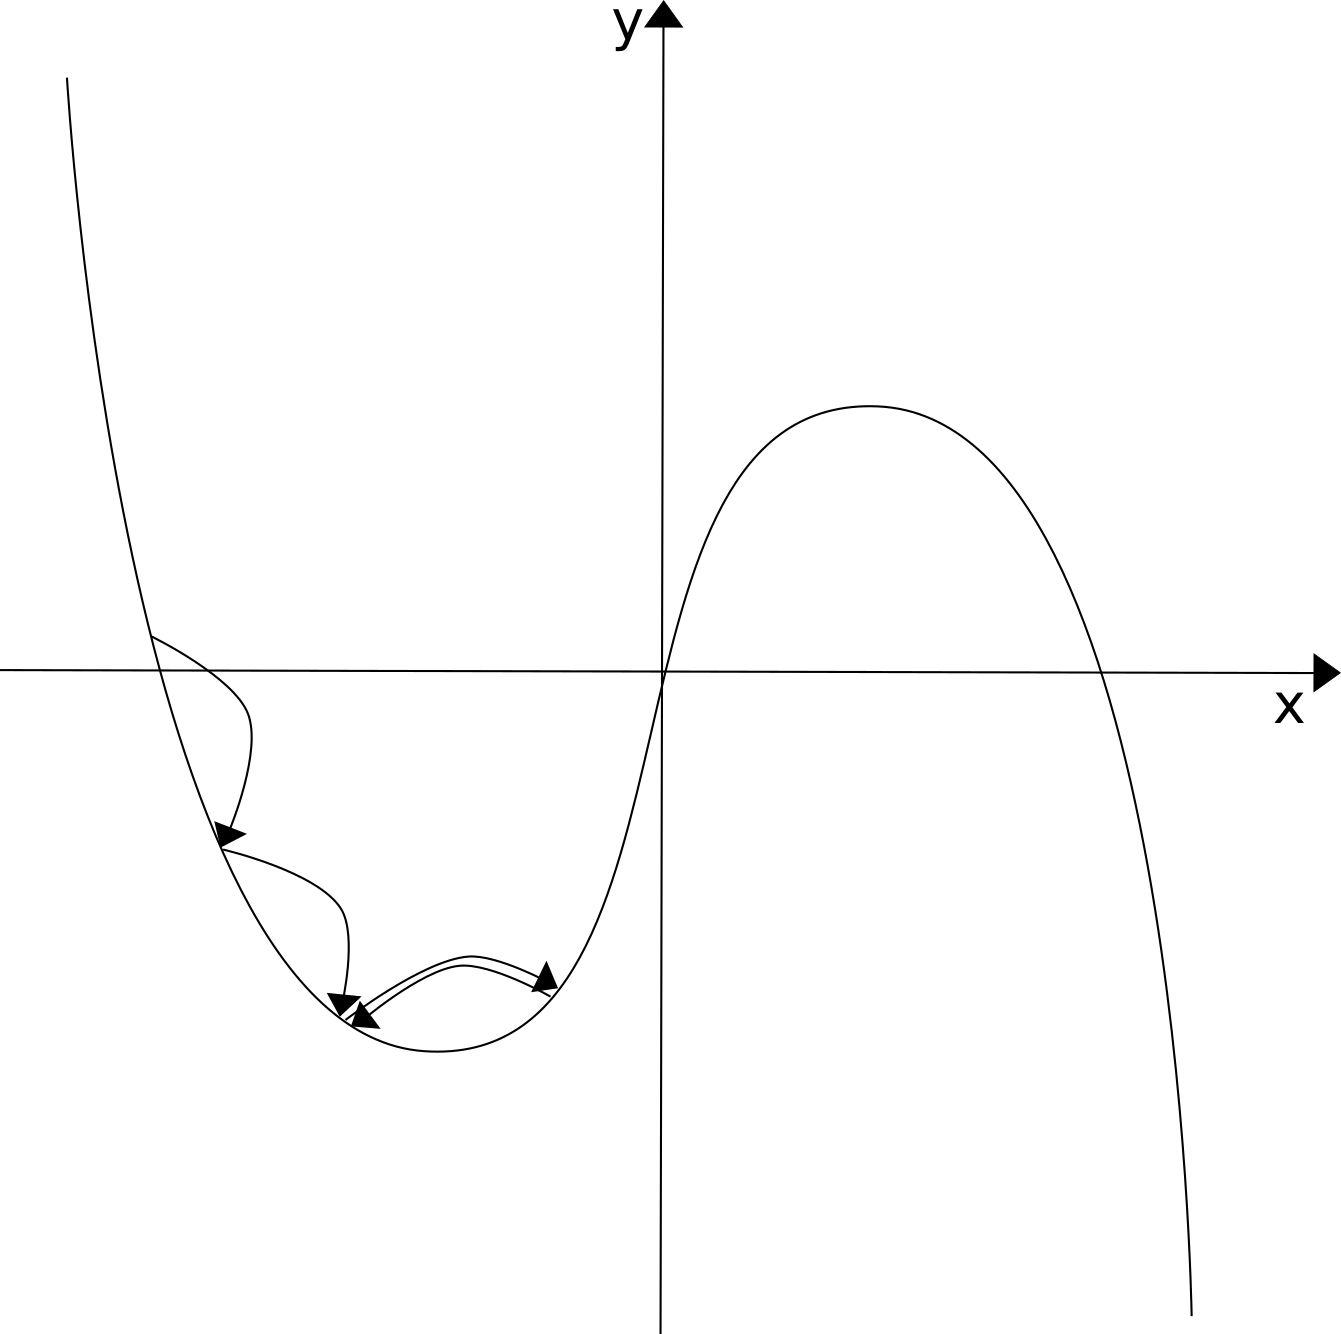
\includegraphics[width=0.4\linewidth]{../graphics/gdf_big_lr.png}
	\end{center}
	\caption{$\eta$ ist hier zu groß gewählt, sodass das Minimum stets übersprungen wird.}
	\label{Learning_Rate_Graphic}
\end{figure}
\\
Abbildung \ref{Learning_Rate_Graphic} stellt dar, wieso das Minimum nicht erreicht werden kann, falls die Lernrate zu groß gewählt wurde. Es ist zu sehen, dass der Parameter immer gleich viel geändert und dabei das Minimum übersprungen wird, da die Lernrate konstant zu groß ist. Dieses Problem kann behoben werden, indem eine adaptive Lernrate verwendet wird. Dabei verringert sich die Lernrate im Laufe des Lernprozesses, sodass zu Beginn die Vorzüge des schnellen Lernens genutzt werden können und am Ende trotzdem ein hoher Grad an Präzision erreicht werden kann.
\subsection{Verschiedene Layerarten}
Mit Hilfe von maschinellem Lernen lassen sich eine Vielzahl von Aufgaben bewältigen. Entsprechend komplex müssen Neuronale Netze aber auch sein. Daher ist es notwendig, Neuronen zu entwickeln, die andere Fähigkeiten aufweisen, als das einfache im sogenannten \glqq Linear Layer'' verwendete Neuron. Da man in der Regel nur eine Art von Neuronen in einem Layer verwendet, wird das gesamte Layer nach der verwendeten Neuronenart benannt. Die unten beschriebenen Layerarten werden vor allem in einer Klasse von neuronalen Netzen verwendet, die als \glqq Convolutional Neural Networks'' bezeichnet werden. Sie werden meist im Bereich der komplexen fragmentbasierten Bilderkennung eingesetzt, da sie besonders gut geeignet sind, um Kanten oder gewisse Teile eines Bildes wie zum Beispiel Merkmale eines Gesichtes zu erkennen.
\subsubsection{Convolutional Layers}
Convolutional Layers weisen eine fundamental andere Funktionsweise als lineare Layers auf. Sie nehmen zwar ebenfalls rationale Zahlen an und geben rationale Zahlen aus \footnote{Im Folgenden werden zweidimensionale convolutional Layers betrachtet, da diese einfacher vorstellbar sind. Sie nehmen dann eine Matrix rationaler Zahlen an und geben auch eine Matrix rationaler Zahlen aus. Dies korrespondiert mit dem Anwendungsbereich der Erkennung von schwarz-weiß-Bildern.}, berechnen die Ausgabe jedoch nicht nur mit Hilfe einer Aktivierungsfunktion, sondern unter der Verwendung sogenannter \glqq Filter''. Diese Filter sind eine $m\times n$ große Matrix, die auch als \glqq Kernel'' bezeichnet wird. Der Kernel wird dabei über die Eingabematrix bewegt (daher der Name convolution) und erzeugt eine Ausgabematrix. Dafür wird der betrachtete Abschnitt der Eingabematrix $A$ und des Kernels $B$ skalar multipliziert, wobei das Skalarprodukt als Frobenius-Skalarprodukt, also als
\begin{equation*}
	\langle A, B\rangle=\sum_{i=1}^{m}\sum_{j=1}^{n}a_{ij}b_{ij}
\end{equation*} 
definiert ist. Die Matritzen werden also komponentenweise multipliziert und diese Produkte dann summiert.\newline
Dies ist in Abbildung \ref{Convolution_illustration} verbildlicht.
\begin{figure}[h]
	\begin{center}
	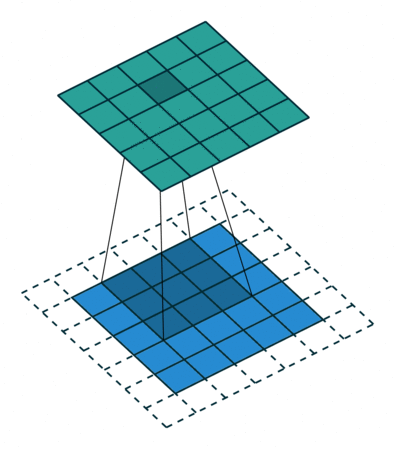
\includegraphics[width=0.2\linewidth]{../graphics/conv/conv008.png}
	\end{center}
	\caption[Eine Verbildlichung der Vorgänge in einem convolutional Layer\newline
	Aus einer Animation von\newline
	https://github.com/vdumoulin/conv\_arithmetic/blob/master/README.md\\
	Vincent Dumoulin, Francesco Visin - A guide to convolution arithmetic for deep learning (BibTeX)]{Eine Verbildlichung der Vorgänge in einem convolutional Layer. Das blaue Raster stellt die Eingabe dar, das grüne die Ausgabe.}
	\label{Convolution_illustration}
\end{figure}
Ein Filter kann ganz verschiedene Werte aufweisen. So können Filter der Form 
\begin{figure}[h]
	\begin{minipage}{0.2\linewidth}
		\centering
		\begin{equation*}
			\begin{bmatrix}
			-1 & -1 & -1\\
			1 & 1 & 1\\
			0 & 0 & 0
			\end{bmatrix}
		\end{equation*}
		\caption{Erkennt obere horizontale Kanten}
	\end{minipage}
	\hfill
	\begin{minipage}{0.2\linewidth}
		\centering
		\begin{equation*}
			\begin{bmatrix}
			-1 & 1 & 0\\
			-1 & 1 & 0\\
			-1 & 1 & 0
			\end{bmatrix}
		\end{equation*}
		\caption{Erkennt linke vertikale Kanten}
	\end{minipage}
	\hfill
	\begin{minipage}{0.2\linewidth}
		\centering
		\begin{equation*}
			\begin{bmatrix}
			0 & 0 & 0\\
			1 & 1 & 1\\
			-1 & -1 & -1
			\end{bmatrix}
		\end{equation*}
		\caption{Erkennt untere horizontale Kanten}
	\end{minipage}
	\hfill
	\begin{minipage}{0.2\linewidth}
		\centering
		\begin{equation*}
			\begin{bmatrix}
			0 & 1 & -1\\
			0 & 1 & -1\\
			0 & 1 & -1
			\end{bmatrix}
		\end{equation*}
		\caption{Erkennt rechte vertikale Kanten}
	\end{minipage}
\end{figure}
\newline
beispielsweise zur einfachen Kantenerkennung genutzt werden. Zur Veranschaulichung wurden diese Filter auf das Beispielbild in Abbildung \ref{Filter_Example_raw} angewandt. Das Ergebnis ist in Abbildung \ref{Filter_output dargestellt} dargestellt.
\begin{figure}[h]
	\begin{center}
		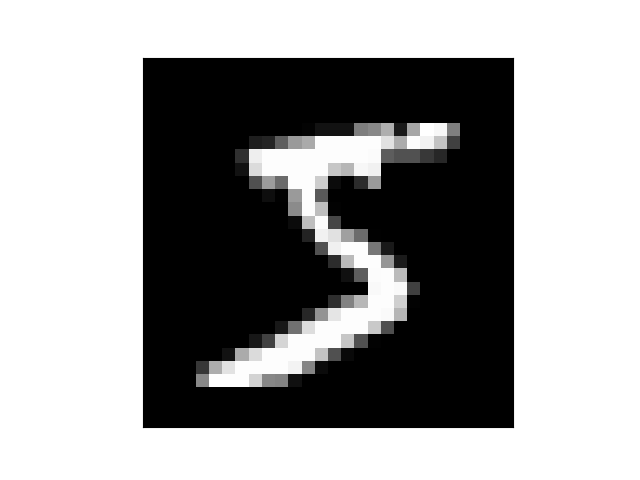
\includegraphics[width=0.5\linewidth]{../graphics/mnist_5/mnist_5_raw.png}
		\caption{Das Beispielbild aus dem Mnist Datensatz}
		\label{Filter_Example_raw}
	\end{center}
\end{figure}
\begin{figure}[h]
	\begin{minipage}{0.2\linewidth}
		\centering
		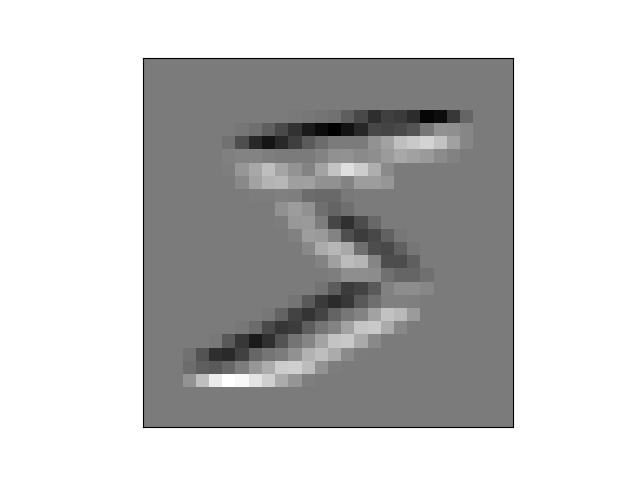
\includegraphics[width=\linewidth]{../graphics/mnist_5/conv_only/mnist_5_upper_edges.png}
	\end{minipage}
	\hfill
	\begin{minipage}{0.2\linewidth}
		\centering
		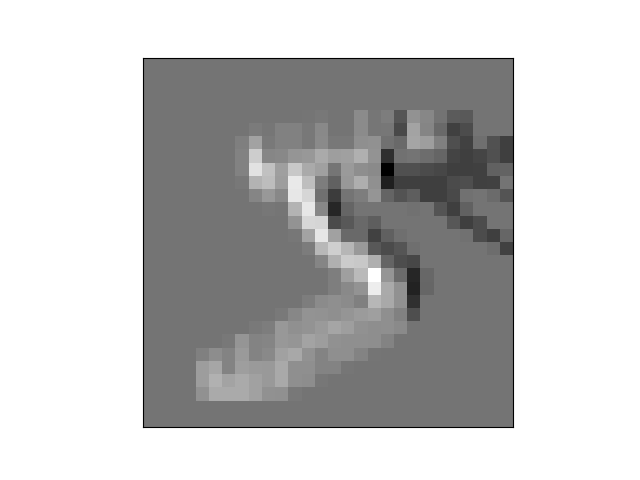
\includegraphics[width=\linewidth]{../graphics/mnist_5/conv_only/mnist_5_left_edges.png}
	\end{minipage}
	\hfill
	\begin{minipage}{0.2\linewidth}
		\centering
		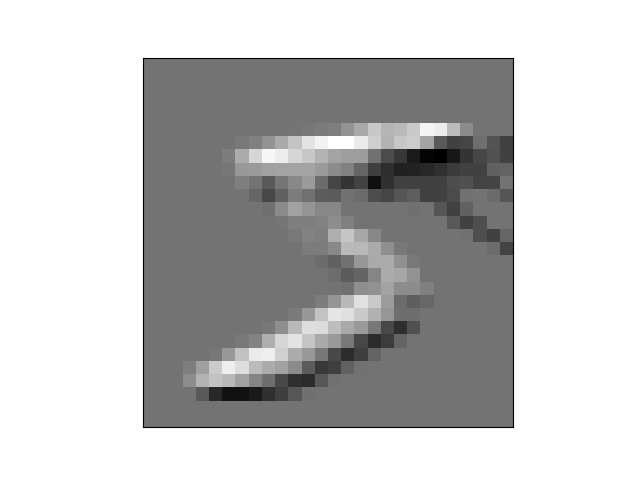
\includegraphics[width=\linewidth]{../graphics/mnist_5/conv_only/mnist_5_lower_edges.png}
	\end{minipage}
	\hfill
	\begin{minipage}{0.2\linewidth}
		\centering
		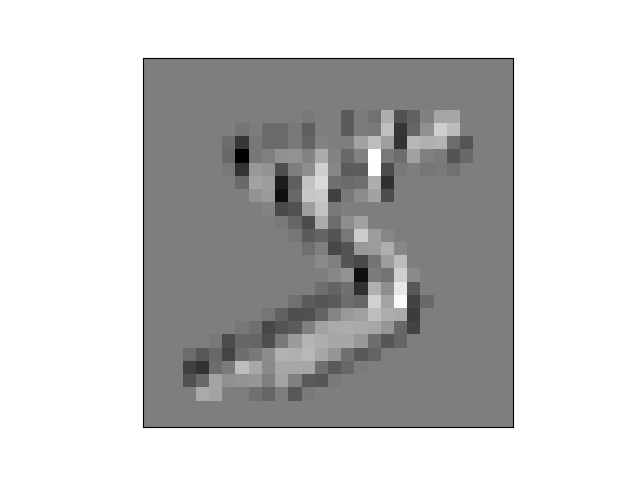
\includegraphics[width=\linewidth]{../graphics/mnist_5/conv_only/mnist_5_right_edges.png}
	\end{minipage}
\caption{Die jeweils oben stehenden Filter wurden auf das Beispielbild angewandt.}
\label{Filter_output dargestellt}
\end{figure}
Der jeweils dunkel dargestellte Bereich kann als das identifiziert werden, was vom Convolutional Layer als Kante erkannt wurde. Hier werden eindeutige Einschränkungen deutlich: Es kann nur als Kante erkannt werden, was auch eindeutig senkrecht oder waagerecht ist. Außerdem kann es zu Fehlentscheidungen kommen.\\
Die Kernels werden natürlich nicht per Hand initialisiert und angepasst, sondern setzen sich aus Parametern zusammen, die im Laufe des Lernprozesses durch das Netz anpassbar sind. Das Netz kann also die Filtermatrix selber verändern. Die Filter werden meist mit Zufallswerten initialisiert und dann während des Lernens  angepasst. Ferner muss ein Kernel auch nicht immer drei Einheiten breit sein, sondern kann jede Größe $\ge2$ annehmen. Je nachdem, wie sich der Kernel über die Eingabematrix bewegt, ist außerdem ein sogenanntes \glqq Padding'' nötig, da gegebenenfalls Werte betrachtet werden müssten, die nicht in der Eingabematrix liegen. In der Regel werden daher alle Werte, die nicht in der Eingabematrix vorhanden sind, durch 0 ersetzt. Das Padding ist in Abbildung \ref{Convolution_illustration} in der Eingabematrix weiß dargestellt. Es ist eine Art \glqq Rand aus Nullen'', der um das Bild gelegt wird.
\\ 
\\
Hintereinander können Convolutional Layers auch ganze Elemente eines Bildes erkennen. Erkennt das erste Layer wie oben gezeigt beispielsweise Kanten, so kann das Layer darauf Kombinationen aus diesen, wie beispielsweise Ecken oder Winkel, erkennen. Wie gefilterte Bilder für sogenannte \glqq High-Level-Features'' aussehen können, ist in Abbildung \ref{HL_features_conv} dargestellt. Die Ausgabebilder von Convolutional Layers werden als \glqq Feature map'' bezeichnet.
\begin{figure}[h]
	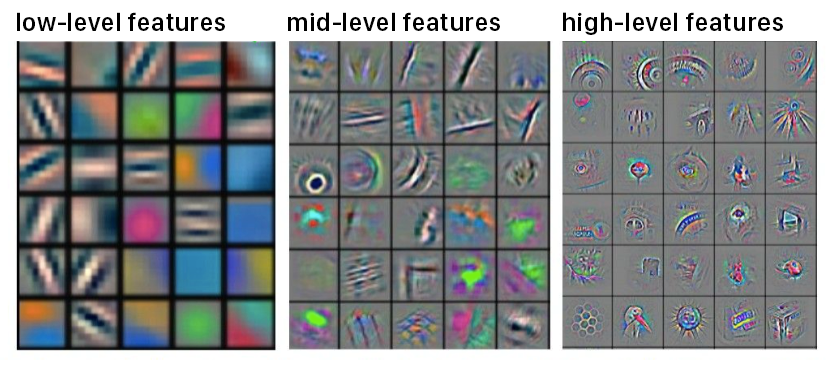
\includegraphics[width=\linewidth]{../graphics/features.png}
	\caption[Beispiele für low-, mid- und high-level Features in Convolutional Neural Nets\newline
	Quelle: https://tvirdi.github.io/2017-10-29/cnn/]{Beispiele für low- mid- und high-level Features in Convolutional Neural Nets}
	\label{HL_features_conv}
\end{figure}
\\
Das bemerkenswerte an Convolutional Layers ist vor allem, dass durch ähnliche Optimierungsalgorithmen auch hier maschinelles Lernen möglich ist, sich ein neuronales Netz diese Filter also selbstständig beibringen kann.
\subsubsection{Pooling Layers}
Pooling Layers werden ebenfalls hauptsächlich in Convolutional Neural Networks verwendet. Sie werden nach Convolutional Layers genutzt, um das Ausgabebild herunterzutakten, also verlustbehaftet zu komprimieren. Dabei wird die Feature Map im wesentlichen zusammengefasst, um die Datenmenge, die das folgende Convolutional Layer erhält, zu reduzieren und sie Verschiebungen im Originalbild gegenüber immuner zu machen. Das ist notwendig, weil die Convolutional Layers die Features lokal sehr begrenzt erkennen und daher eine kleine Verschiebung des Originalbildes zur Folge haben kann, dass im folgenden Convolutional Layer die Kombination der Features gegebenenfalls nicht richtig erkannt wird. Das Pooling Layer kann diesem Effekt entgegenwirken, indem es die Features zusammenfasst. So kann aus einer ganzen Kante beispielsweise ein einziger Pixel werden.\\
Es werden im Wesentlichen zwei Techniken zum Pooling eingesetzt. 
\begin{enumerate}
	\item Max Pooling (Abbildung \ref{Maxpool})
	\item  Average-Pooling (Abbildung \ref{AvgPool})
\end{enumerate}
Sie unterscheiden sich darin, wie die zu komprimierenden Werte miteinander verrechnet werden, sind ansonsten jedoch identisch.\\
Beim Pooling wird die Eingabematrix in Submatrizen partitioniert\footnote{Hier ist die mengentheoretische Partitionierung gemeint. Eine Menge wird in nicht leere Teilmengen unterteilt, sodass jedes Element der Ausgangsmenge in genau einer der Teilmengen enthalten ist.}. Jede Submatrix stellt später einen Pixel in der Ausgabematrix dar. Hier unterscheiden sich jetzt Max- und Avarage- Pooling. Beim Max Pooling ist der neue Wert der höchste Wert aus dieser Submatrix, beim Avarage Pooling wird der Durchschnitt aller Werte der Submatrix gebildet und als neuer Wert verwendet.
\begin{figure}[h]
	\centering
	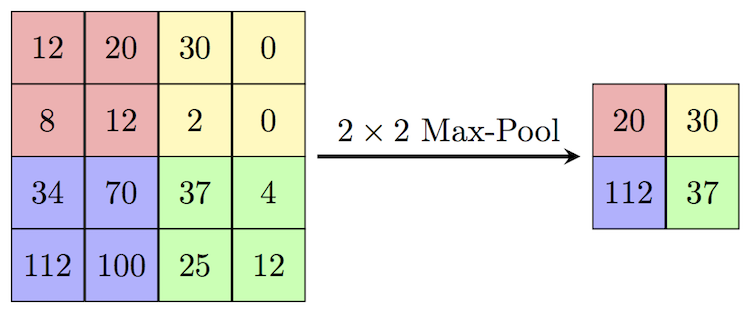
\includegraphics[width=0.7\linewidth]{../graphics/MaxpoolSample2.png}
	\caption[Max Pooling mit $2\times2$ großen Submatrizen\newline
	Quelle: https://computersciencewiki.org/index.php/Max-pooling\_/\_Pooling\\
	CC BY NC SA Lizenz]{Max Pooling mit $2\times2$ großen Submatrizen}
	\label{Maxpool}
\end{figure}
\begin{figure}[h]
	\centering
	\includegraphics[width=0.7\linewidth]{../graphics/Average-Pooling-Example.png}
	\caption[Average-Pooling mit $2\times2$ großen Submatrizen\newline
	Aus: Dominguez-Morales, Juan Pedro. (2018). Neuromorphic audio processing through real-time embedded spiking neural networks. Abbildung 33]{Average-Pooling mit $2\times2$ großen Submatrizen}
	\label{AvgPool}
\end{figure}
\\
Die Dimension der Submatrizen beträgt meist $2\times2$. In Abbildung \ref{Pooling_Mnist} ist dargestellt, wie Pooling konkret auf das im letzten Abschnitt beschriebene Bild angewandt aussieht. Dafür sind in der ersten Zeile die $28\times28$ Pixel großen Bilder dargestellt, die das Convolutional Layer mit Hilfe der Kantenerkennungsfilter berechnet hat. In Zeile zwei wurde auf die jeweils darüber stehenden Bilder Max Pooling angewandt, in Zeile drei auf dieselben Bilder Average-Pooling. Die Bilder sind nach dem Pooling $14\times14$ Pixel groß.
\begin{figure}[h]
	\begin{minipage}{0.2\linewidth}
		\centering
		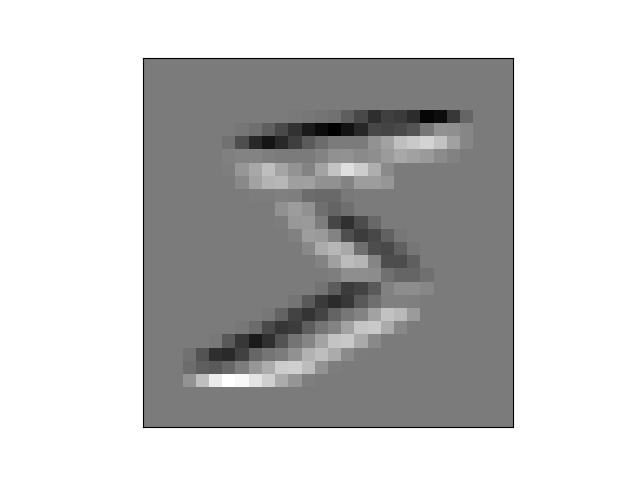
\includegraphics[width=\linewidth]{../graphics/mnist_5/conv_only/mnist_5_upper_edges.png}
	\end{minipage}
	\hfill
	\begin{minipage}{0.2\linewidth}
		\centering
		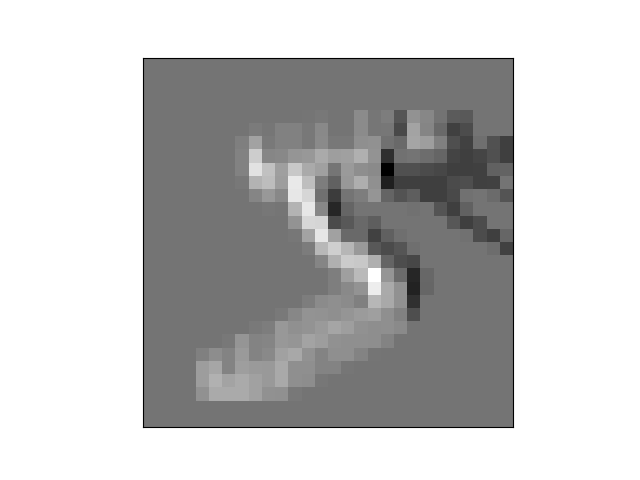
\includegraphics[width=\linewidth]{../graphics/mnist_5/conv_only/mnist_5_left_edges.png}
	\end{minipage}
	\hfill
	\begin{minipage}{0.2\linewidth}
		\centering
		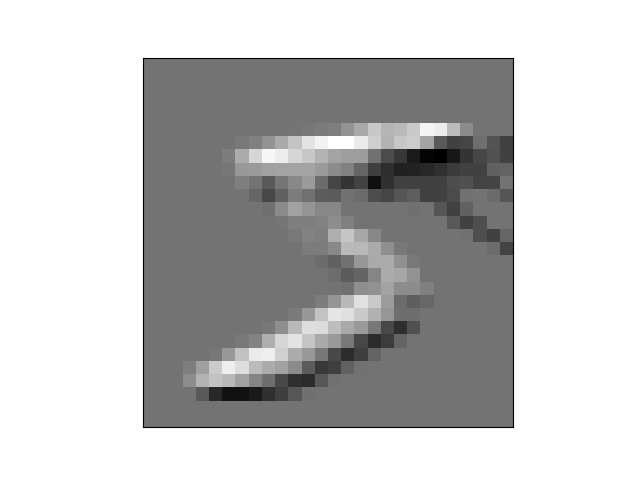
\includegraphics[width=\linewidth]{../graphics/mnist_5/conv_only/mnist_5_lower_edges.png}
	\end{minipage}
	\hfill
	\begin{minipage}{0.2\linewidth}
		\centering
		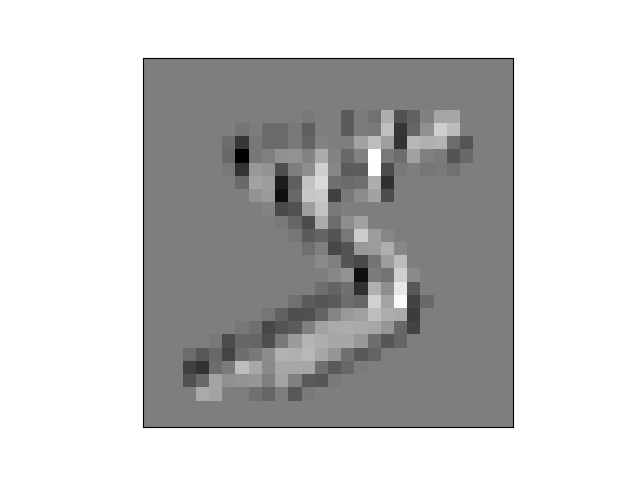
\includegraphics[width=\linewidth]{../graphics/mnist_5/conv_only/mnist_5_right_edges.png}
	\end{minipage}
\\
	\begin{minipage}{0.2\linewidth}
	\centering
	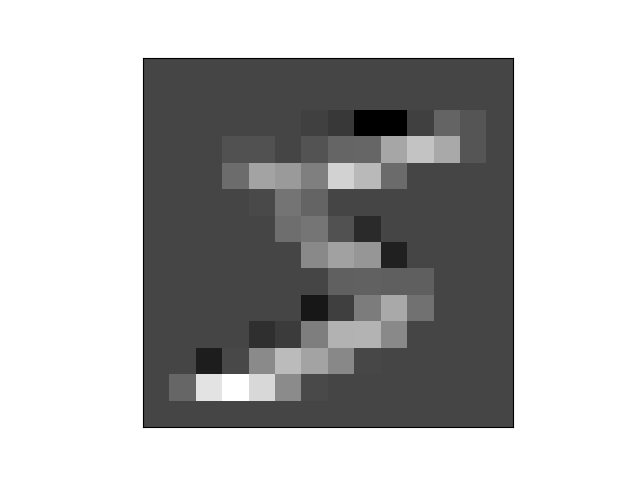
\includegraphics[width=\linewidth]{../graphics/mnist_5/conv_pool/upper_horiz_pooled.png}
\end{minipage}
\hfill
\begin{minipage}{0.2\linewidth}
	\centering
	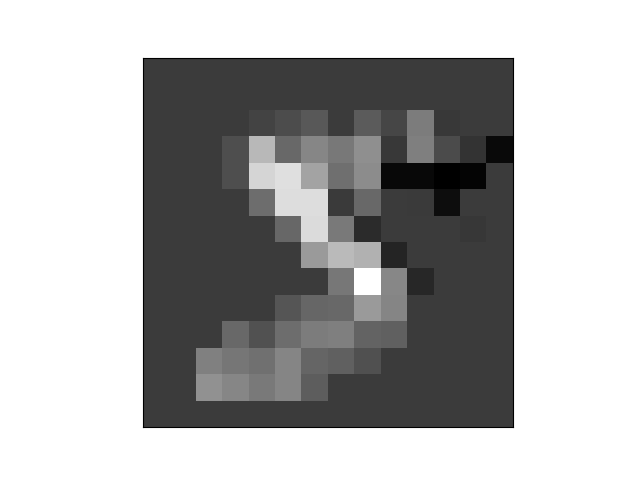
\includegraphics[width=\linewidth]{../graphics/mnist_5/conv_pool/left_vert_pooled.png}
\end{minipage}
\hfill
\begin{minipage}{0.2\linewidth}
	\centering
	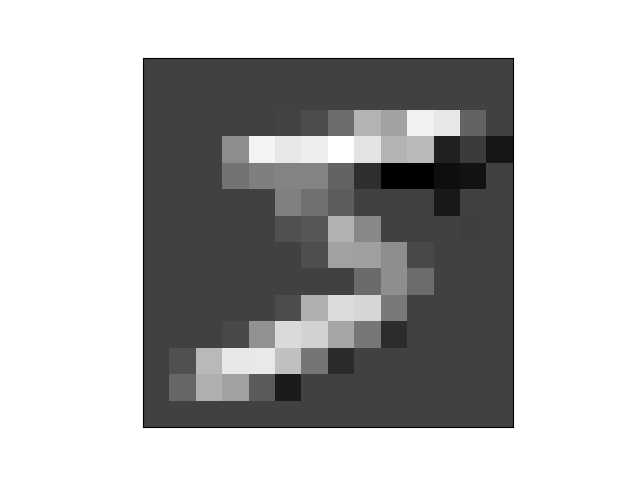
\includegraphics[width=\linewidth]{../graphics/mnist_5/conv_pool/lower_horiz_pooled.png}
\end{minipage}
\hfill
\begin{minipage}{0.2\linewidth}
	\centering
	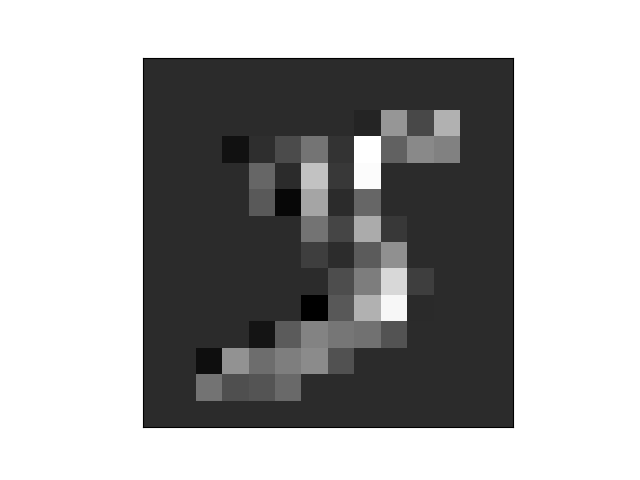
\includegraphics[width=\linewidth]{../graphics/mnist_5/conv_pool/right_vert_pooled.png}
\end{minipage}
\\
	\begin{minipage}{0.2\linewidth}
	\centering
	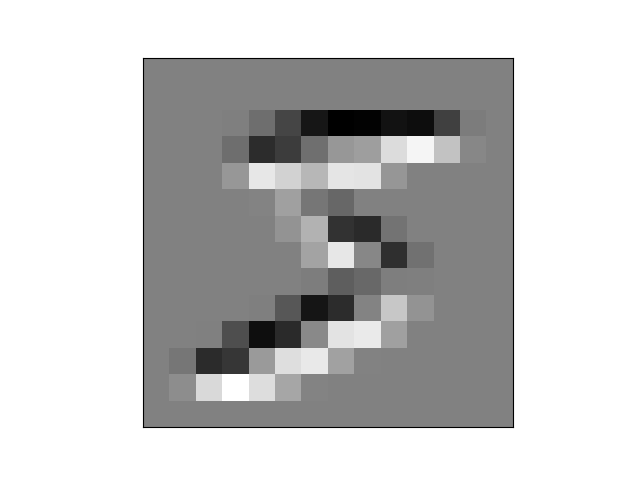
\includegraphics[width=\linewidth]{../graphics/mnist_5/conv_pool/upper_horiz_avgpooled.png}
\end{minipage}
\hfill
\begin{minipage}{0.2\linewidth}
	\centering
	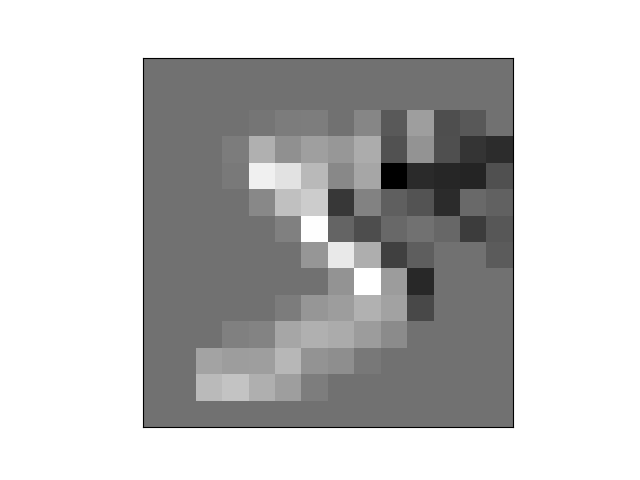
\includegraphics[width=\linewidth]{../graphics/mnist_5/conv_pool/left_vert_avgpooled.png}
\end{minipage}
\hfill
\begin{minipage}{0.2\linewidth}
	\centering
	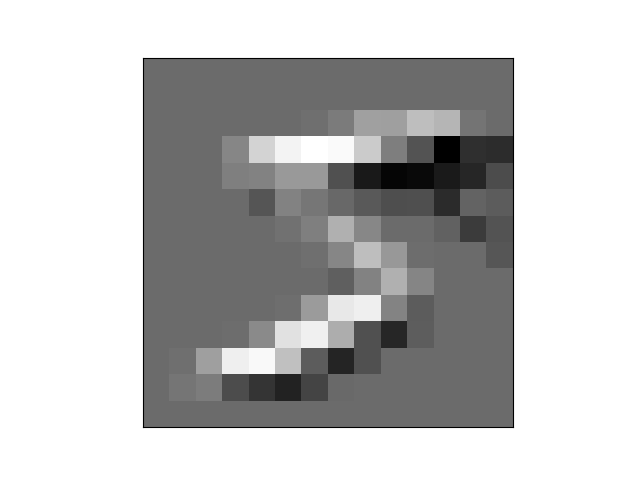
\includegraphics[width=\linewidth]{../graphics/mnist_5/conv_pool/lower_horiz_avgpooled.png}
\end{minipage}
\hfill
\begin{minipage}{0.2\linewidth}
	\centering
	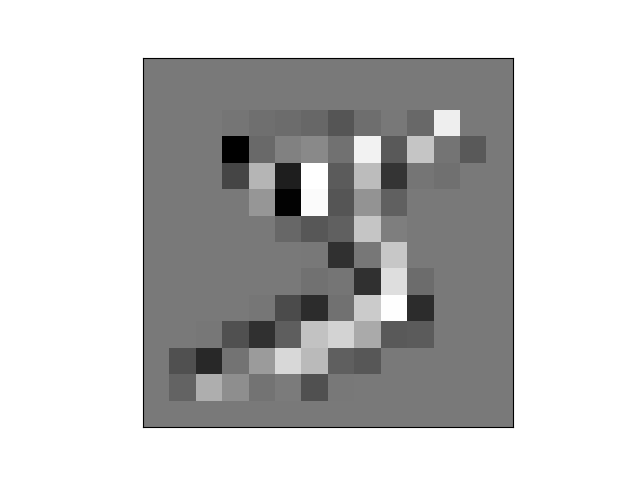
\includegraphics[width=\linewidth]{../graphics/mnist_5/conv_pool/right_vert_avgpooled.png}
\end{minipage}
\caption{Gegenüberstellung von Max- und Average-Pooling}
\label{Pooling_Mnist}
\end{figure}
\\
\section{PyTorch}
Pytorch ist ein von der Facebook Research Group entwickeltes Framework für maschinelles Lernen in Python. Es ermöglicht Programmierern, maschinelles Lernen einfach und hochoptimiert umzusetzen. Dafür stellt es unter anderem eine Schnittstelle für Grafikkarten bereit und liefert viele Funktionen, die oft benötigt werden. So muss beispielsweise die Gradientenberechnung oder die Berechnung der Fehlerfunktion nicht in jedem Projekt erneut implementiert werden. Die Grundlage der Pytorch Library ist der Datentyp \glqq Tensor''. Dabei handelt es sich im wesentlichen um eine Matrix, die optimierte Funktionen für maschinelles Lernen aufweist und auf Grafikkarten transferiert werden kann. Alle Daten werden in Form dieser Tensoren gespeichert und verarbeitet. Sollen also Bilder erkannt werden, müssen diese erst zu Tensoren konvertiert werden. Neben den Fehlerfunktionen und der Gradientenberechnung ist besonders die Einfachheit, mit der ein Netz in Pytorch definiert werden kann, bezeichnend. Pytorch ermöglicht es also, dass die Entwicklung auf die Logik selber fokussiert sein kann und trotzdem komplexe mathematische Funktionen verwendet werden können. Häufig genannte Alternativen zu Pytorch sind die Frameworks \glqq Tensorflow'' oder \glqq Keras''. Tensorflow wird von Google entwickelt und ist auch für andere Sprachen als Python verfügbar.
\subsection{Datenvorbereitung}
Wie bereits erwähnt, müssen die Daten erst vorbereitet werden. Dies kann unter Umständen das größte Problem bei einem Projekt, das maschinelles Lernen involviert, darstellen, da die Datenvorbereitung sehr komplex werden kann. In einem einfachen Fall liegt der Datensatz bereits in Pytorchs interner Datenlibrary \glqq Torchvision'' vor und muss nur noch geladen werden. Im komplexesten Fall kann es allerdings notwendig werden, mehrere sogenannte \glqq Transforms'' auf die Daten anzuwenden. Das sind Funktionen, die die Daten verändern. Sie schneiden beispielsweise das Eingabebild zu, normalisieren es oder wenden eine vollständig selbst definierte Funktion darauf an.\\
In ein neuronales Netz können immer nur Bilder der gleichen Größe gegeben werden, da die Größe der Eingabetensoren konstant ist und die Form des Eingabelayers definiert. Ist also ein Datensatz gegeben, in dem zum Beispiel  einige Bilder im Hoch- und einige im Querformat vorliegen, müssen diese erst durch Zuschneiden und Verschieben auf eine Größe gebracht werden. Auch dafür lassen sich Transforms verwenden. Liegen die Daten allerdings nicht als Bilder vor, müssen gegebenenfalls angepasste Algorithmen angewandt werden, um diese Daten zu Tensoren zu konvertieren.\\
Aufgrund der Vielseitigkeit von PyTorch ist es ebenfalls möglich, andere Libraries einzubinden, um vor der Konvertierung der Bilder zu einem Tensor zum Beispiel einen Kantenerkennungsalgorithmus darauf anzuwenden. Im einfachsten Fall stellt sich das Laden der Daten wie in Abbildung \ref{MNIST_Dataloader_Code} dar.
\newpage
\begin{figure}[h]
	\begin{minted}[
	frame=lines,
	framesep=2mm,
	baselinestretch=1.2,
	fontsize=\footnotesize,
	linenos,
	autogobble
	]{python}
		from torchvision import transforms, datasets
	
		train = datasets.MNIST('./datasets', train=True, download=True,
		transform=transforms.Compose([
			transforms.ToTensor()
		]))
		
		test = datasets.MNIST('./datasets', train=False, download=True,
		transform=transforms.Compose([
			transforms.ToTensor()
		]))
		
		trainset = torch.utils.data.DataLoader(train, batch_size=200, shuffle=True)
		testset = torch.utils.data.DataLoader(test, batch_size=10, shuffle=False)
	\end{minted}
	\caption{Der Code zum Laden des MNIST Datensatzes}
	\label{MNIST_Dataloader_Code}
\end{figure}
Der Code lädt zwei Datensätze. Einen zum Testen und einen zum Trainieren. Anschließend wird aus diesen je ein DataLoader erstellt, um über die Daten iterieren zu können. In Zeile 1 werden dafür zunächst alle nötigen Funktionen importiert. Die Zeilen 3 bis 6 sind für das eigentliche Laden der Daten zuständig.
Die Funktion \mintinline{python}{datasets.MNIST()} nimmt dabei vier Parameter an:
\begin{enumerate}
	\item \mintinline{python}{./datasets} Dieser Parameter gibt den Speicherort für den heruntergeladenen Datensatz an
	\item \mintinline{python}{train} Dieser Booleanparameter gibt an, ob es sich bei diesem Datensatz um den Trainingsdatensatz oder um den Testdatensatz handeln soll.
	\item \mintinline{python}{download} Mit diesem Parameter wird festgelegt, ob der Datensatz heruntergeladen werden, oder jedesmal erneut aus dem Internet abgerufen werden soll.
	\item \mintinline{python}{transform} Hier werden die Transforms angegeben, die auf die geladenen Daten angewandt werden sollen. In diesem Fall wurde der Ansatz\\ \mintinline{python}{transforms.Compose([transforms.ToTensor()])} gewählt.\\ \mintinline{python}{transforms.Compose()} ist dabei dafür verantwortlich, die Transforms im Array zu kaskadieren, also nacheinander auf die Eingabedaten anzuwenden. \\
	\mintinline{python}{transforms.ToTensor()} ist der häufigste Transform. Er wird eingesetzt, um Bilddaten in einen Tensor umzuwandeln.
\end{enumerate}
In Zeile 13 wird dann der DataLoader erstellt. Er nimmt folgende Parameter an:
\begin{enumerate}
	\item Der erste Parameter ist der Datensatz, aus dem der DataLoader erstellt werden soll
	\item \mintinline{python}{batch_size} Ist ein Parameter, der eine ganz fundamentale Variable beim maschinellen Lernen durch neuronale Netze festlegt: die Batchsize.\\
	Die Tensoren werden nämlich nicht einzeln, sondern in sogenannten minibatches in das Netz gegeben. Es wird mit Durchschnittswerten über diese Tensoren in einer Minibatch gerechnet. Dies dient der Reduktion der Rechenzeit. Batching kann veranschaulicht werden, indem man sich vorstellt, dass die \glqq Eingabebilder'' hintereinander geklebt und alle gleichzeitzig betrachtet werden. Die Batchsize gibt dann analog an, wie viele Bilder hintereinander geklebt werden. Je höher die Batchsize, desto höher ist die Speicherauslastung auf der Grafikkarte und desto ungenauer ist das Ergebnis, da über mehr Werte der Durchschnitt gerechnet wird. Mit höherer Batchsize sinkt allerdings auch die Rechenzeit massiv.
	\item \mintinline{python}{shuffle} gibt lediglich an, ob die Reihenfolge der Daten randomisiert werden soll. Dies ist, wie am Anfang bereits erwähnt, ein sehr nützlicher Parameter, um overfitting vorzubeugen.
\end{enumerate}
Über den entstandenen DataLoader kann jetzt in einer konventionellen Schleife iteriert werden, da die Klasse DataLoader die MagicMethod \mintinline{python}{__iter__} implementiert. Der DataLoader gibt dabei Tupel der Form (Batch von Bildern als Tensoren, Batch von Labels als Klassenindices) zurück.
\subsection{Definieren des Netzes}
Das Definieren des Netzes ist in Pytorch bereits sehr einfach möglich, bietet dennoch extreme individuelle Anpassungsmöglichkeiten. Um ein Netz zu definieren, muss zunächst eine neue Klasse erstellt werden, die Subklasse von \mintinline{python}{nn.Module} ist. Im Konstruktor wird dann angegeben, welche Layers das Netz haben soll. Es muss außerdem die Methode \mintinline{python}{forward(self, x)} implementiert werden. Diese spezifiziert, wie mit den Daten innerhalb des Netzes verfahren wird. Eine möglichst einfache Definition  eines Netzes ist in Abbildung \ref{Net_simple_definition} gegeben.
\newpage
\begin{figure}[h]
	\begin{minted}[
	frame=lines,
	framesep=2mm,
	baselinestretch=1.2,
	fontsize=\footnotesize,
	linenos,
	autogobble
	]{python}
	class Net(nn.Module):
		def __init__(self):
			super().__init__()
			self.fc0 = nn.Linear(28 * 28, 64)
			self.fc1 = nn.Linear(64, 120)
			self.fc2 = nn.Linear(120, 10)
	
		def forward(self, x):
			x = F.relu(self.fc0(x))
			x = F.relu(self.fc1(x))
			x = self.fc2(x)
			return F.log_softmax(x)
	
	\end{minted}
	\caption{Code, um ein einfaches Netz in Pytorch zu definieren}
	\label{Net_simple_definition}
\end{figure}
Dieses Netz hat nur drei Layers: Ein Eingabelayer (\mintinline{python}{fc0}), das genau die Größe der Eingabedaten ($28\times28$) aufweist, ein hidden Layer (\mintinline{python}{fc1}), das 64 Skalare annimmt und 120 Skalare ausgibt und ein Ausgabelayer (\mintinline{python}{fc2}), das 120 Skalare annimmt und 10 ausgibt. Dass \mintinline{python}{fc2} 10 Ausgabeneuronen besitzt, ist kein Zufall, sondern liegt darin begründet, dass dieses Klassifizierungsnetz genau 10 Klassen unterscheiden soll. Die Größe von \mintinline{python}{fc1} ist jedoch völlig frei gewählt. Es ist allerdings wichtig, zu beachten, dass die Layers die Daten auch aneinander weitergeben können. Ein Layer muss also stets so viele Ausgaben aufweisen, wie das Layer, an das die Daten weitergegeben werden sollen, Eingaben besitzt.\\
Die \mintinline{python}{forward(self, x)} Funktion definiert, wie die Daten innerhalb des Netzes weitergegeben werden sollen. Hier werden sie erst in \mintinline{python}{fc0} gegeben, dann wird auf die Ausgabe aus \mintinline{python}{fc0} die Aktivierungsfunktion \glqq ReLu'' (REctified Linear Unit) angewandt. Die Ausgabe daraus wird dann in das hidden Layer \mintinline{python}{fc1} gegeben, und die Aktivierungsfunktion wird erneut angewandt. Im Output Layer geschieht dies nicht. Abschließend wird die Ausgabe von \mintinline{python}{F.log_softmax} zurück gegeben. Dies wendet erst einen SoftMax und dann einen Logarithmus auf die Daten an, \cite{6} um diese zu normalisieren und ist in Klassifizierungsnetzwerken oft nötig, um sogenannte \glqq One hot Vectors'' zu erstellen. Herkömmliche Ausgabevektoren haben einen Wert für jede Klasse und geben an, wie wahrscheinlich das Netz die Eingabedaten dieser Klasse zuordnet. In One hot Vektoren ist immer der höchste Wert 1 und alle anderen Werte sind 0.\\
Da die Netze als Klassen definiert werden und der netzinterne Datenverkehr in der \mintinline{python}{forward(self, x)} Funktion abläuft, sind neuronale Netze in Pytorch also sehr anpassbar. So wäre es beispielsweise kein Problem, zwischen Input und hidden Layer die Daten mit 2 zu multiplizieren (dafür würde man zwischen Zeile 9 und 10 den Code \glqq\mintinline{python}{x = x * 2}'' einfügen), auch wenn dies in den meisten Anwendungsbereichen keinen Sinn ergäbe. Pytorch kombiniert mit dieser Art, Netze zu definieren, also eine umfangreiche Flexibilität mit einfacher Bedienbarkeit.
\subsection{Trainieren des Netzes}
Das Trainieren des Netzes erfolgt in der sogenannten \glqq Training Loop'', also in einer Schleife, die über den Datensatz iteriert. Zumeist steht diese noch in einer Schleife, die über die Epochenzahl iteriert. In der Training loop wird ein Element des Datensatzes gelesen, in das Netz gegeben, die Ausgabe wird mit dem Label verglichen, und schließlich werden die Parameter des Netzes angepasst. Der Code dafür ist in Abbildung \ref{Code_train_loop} dargestellt.
 \begin{figure}[h]
 	\begin{minted}[
 	frame=lines,
 	framesep=2mm,
 	baselinestretch=1.2,
 	fontsize=\footnotesize,
 	linenos,
 	autogobble
 	]{python}
net = Net()

device = torch.device("cuda:0" if torch.cuda.is_available() else "cpu")
print('runnning on %s' % device)
net = net.to(device)

loss_function = nn.CrossEntropyLoss()
optimizer = optim.Adam(net.parameters(), lr=LEARNING_RATE)

for epoch in range(EPOCHS):
	for data in trainset:
		X, y = data
		net.zero_grad() 
		X = X.to(device)
		output = net(X.view(-1, n * n))
		output = output.cpu()
		loss = loss_function(output, y)  
		loss.backward() 
		optimizer.step()  
		
	net = net.cpu()
	torch.save(net, './nets/net_' + str(epoch) + ".pt")
	net = net.to(device)

 	\end{minted}
 	\caption{Code, um das Netz auf einem Datensatz zu trainieren}
 	\label{Code_train_loop}
 \end{figure}
\\
In Zeile 1 wird dafür zunächst das Netz instanziiert. In Zeile 3 und 4 wird bestimmt, ob eine Grafikkarte zum Trainieren verfügbar ist, und diese wird gegebenenfalls genutzt. Auch wird ausgegeben, auf welchem Gerät das Netz trainiert wird. Der Code in Zeile 5 verschiebt das Netz auf die Grafikkarte, um dort mit diesem rechnen zu können. In Zeile 7 wird die Fehlerfunktion definiert, hier der Kreuzentropiefehler. In der nächsten Zeile wird der sogenannte \glqq Optimizer'' instanziiert. Dieser berechnet später die Gradienten und passt die Parameter des Netzes an. Der Optimizer, der hier gewählt wurde, nennt sich \glqq Adam''. Es handelt sich um einen gradientenbasierten Optimierungsalgorithmus, der von Diederik P. Kingma und Jimmy Ba entwickelt wurde \cite{7}. Eine Liste aller implementierten Optimierungsalgorithmen ist in der PyTorch Dokumentation unter https://pytorch.org/docs/stable/optim.html gegeben.\\
In Zeile 10 folgt nun die Schleife, die über die Anzahl der Epochen iteriert, in der nächste Zeile die Train loop. Sie iteriert pro Epoche einmal über den Datensatz. In Zeile 12 werden die Daten entpackt, da diese als Tupel vorliegen. X stellt dabei eine batch von Eingabevektoren dar, y eine Batch von Features. Zeile 13 setzt die Gradienten auf 0 zurück. Dies ist notwendig, da diese sonst aufsummiert würden. Die Parameter würden also nicht nur den Gradienten aus diesem Schleifendurchgang entsprechend angepasst werden, sonndern entsprechend zu einer Summe aus allen Gradienten. Das würde das Ergebnis verfälschen. Der Befehl in Zeile 14 verschiebt auch den Eingabevektor auf die Grafikkarte, da alle Daten, mit denen das Netz rechnen soll, erst auf dieser sein müssen. In Zeile 15 wird dann die Ausgabe des Netzes aus den Daten berechnet. Hier wird eine weitere Simplifizierung des Lernprozesses durch PyTorch deutlich: Um eine Ausgabe eines Netzes zu berechnen, reicht der Befehl \mintinline{python}{output = net(input)} völlig aus. \mintinline{python}{X.view(-1, n * n)} wandelt den 2-dimensionalen\footnote{Streng genommen ist der Tensor der Bilder aus dem Datensatz nicht 2, sondern 4-dimensional. Er weist die Dimensionen $Batch\_size\times Kanalanzahl\times n \times n$ auf. Die Kanalanzahl entspricht bei Bildern den Farbkanälen, liegt bei schwarz-weiß Bildern also bei 1 und sonst bei 3 bis 4 für RGBA} Tensor des Eingabebildes in einen Eingabevektor um. Auch hier muss das batching wieder beachtet werden, daher die -1. $n\times n$ stellt nämlich die Größe der Eingabebilder dar und -1 passt den ersten Wert automatisch an den zweiten an, entspricht hier also immer der Batchsize.\\
Nachdem der Ausgabevektor berechnet wurde, wird er zunächst auf die CPU verschoben, da dort der Fehler berechnet wird, und anschließend mit Hilfe der Fehlerfunktion mit dem Label verglichen. Dies geschieht in Zeile 16 und 17.\\ \mintinline{python}{loss.backward()} in Zeile 18 sorgt dann dafür, dass der Optimizer alle Anpassungen berechnet, um sie in Zeile 19 anzuwenden. Der weitere Code dient dazu, jede Epoche das Netz in einer Datei abzuspeichern und somit Sicherungskopien zu erstellen. Dafür muss es erst auf die CPU verschoben werden und danach wieder zurück auf die Grafikkarte.
\subsection{Pytorch und weights and biases}
In dem im Folgenden erläuterten Projekt wurde ein Framework namens \glqq weights and biases'' verwendet. Es erlaubt während des Trainingsprozesses auf einer Seite Parameter des Netzes und wichtige Charakteristika des Lernprozesses sowie Eigenschaften der Hardware zu protokollieren. Da es mit Pytorch gut kompatibel ist, sind hierfür nur wenige Zeilen Code notwendig. Zunächst wird mit\\ \mintinline{python}{wandb.init(project='Beispielprojekt')
} das Projekt initialisiert. Danach muss angegeben werden, welches Netz betrachtet werden soll. Dafür verwendet man, nachdem das Netz initialisiert wurde, den Befehl \mintinline{python}{wandb.watch(model)}, wobei \mintinline{python}{model} der Instanz des Netzes entspricht. Danach kann einfach über\\ 
\mintinline{python}{wandb.log({'loss': loss})} zum Beispiel in der Training loop jedes mal der Fehler mitgeschrieben werden.
\section{Ein Klassifizierungsnetzwerk für handgeschriebene Ziffern}
Die Klassifizierung handgeschriebener Ziffern aus dem MNIST Datensatz stellt etwa die \glqq Hello world'' Aufgabe des maschinellen Lernens dar. Sie ist gut zum Erlernen der verschiedenen Algorithmen geeignet, extrem gut dokumentiert, daher leicht nachvollziehbar und ein Paradebeispiel eines Klassifizierungsproblems. Wenn man sich mit maschinellem Lernen beschäftigt, ist es also sehr wahrscheinlich, dass man zuerst ein Klassifizierungssystem für den MNIST Datensatz programmieren wird.
\subsection{Aufgabe}
Die Aufgabe besteht darin, den die handgeschriebenen Ziffern des MNIST Datensatzes klassifizieren zu können. Das Ziel dabei ist es, mit möglichst wenig Trainingsaufwand eine Genauigkeit von mindestens 97\% zu erreichen. Um dies zu bewältigen, soll ein neuronales Netz in PyTorch programmiert und trainiert werden.
\subsection{Der MNIST Datensatz}
Der MNIST Datensatz ist ein Datensatz aus $28\times28$ Pixel großen Graustufenbildern von handgeschriebenen Ziffern. Er weist 60000 Trainingsbilder und 10000 Testbilder auf und ist ein Teil des EMNIST Datensatzes vom National Institute for Standards and Technology, U.S. Department of Commerce. Der Datensatz ist frei unter http://yann.lecun.com/exdb/mnist/ verfügbar. Die Bilder sind bereits zentriert und normalisiert, was diesen Datensatz besonders geeignet für Einsteiger macht. Die meisten Bilder des Datensatzes sind auch von Menschen einfach zu erkennen, einige sind jedoch sehr schwierig einzuordnen und teilweise kaum als Zahl erkennbar. Aufgrund der Einfachheit der Daten sind durchaus hohe Erfolgsquoten zu erwarten. Diese liegen im Schnitt bei 98\%.
\subsection{Das Netz}\label{sec:das-netz}
Das Netz wurde für diese vergleichsweise unkomplizierte Aufgabe einfach gehalten. Es weist drei hidden Layers auf, besteht insgesamt also aus fünf Layers, die alle klassische lineare, fully connected Layers sind. Die Aktivierungsfunktion ist überall eine ReLu\footnote{ReLu steht für rectified linear unit. Diese Aktivierungsfunktion ist neben den Sigmoid Funktionen ebenfalls eine sehr populäre Aktivierungsfunktion. Sie ist als $f(x)=\max(0,x)$ definiert und ist somit für alle $x\le0$ $0$ und für alle $x>0$ $x$.}, deren Plot in Abbildung \ref{ReLu} dargestellt ist. Da es sich um eine Klassifizierungsaufgabe handelt, hat das Ausgabelayer 10 Ausgabeneuronen, die die 10 Ziffern repräsentieren. Es ist wie in Abbildung \ref{net} dargestellt definiert.
\begin{figure}[h]
 	\begin{minted}[
	baselinestretch=1.2,
	fontsize=\footnotesize,
	linenos,
	autogobble
	]{python}
	class Net(nn.Module):
	def __init__(self):
		super().__init__()
		self.fc1 = nn.Linear(28 * 28, 64)
		self.fc2 = nn.Linear(64, 1260)
		self.fc3 = nn.Linear(120, 120)
		self.fc4 = nn.Linear(120, 64)
		self.fc5 = nn.Linear(64, 10)
	
	def forward(self, x):
		x = F.relu(self.fc1(x))
		x = F.relu(self.fc2(x))
		x = F.relu(self.fc3(x))
		x = F.relu(self.fc4(x))
		x = self.fc5(x)
		return F.log_softmax(x, dim=1)
	\end{minted}
	\caption{Der Code, um das in diesem Projekt genutzte Klassifizierungsnetz zu definieren.}
	 \label{net}
\end{figure}
Das erste Layer nimmt also einen Tensor der Größe $1\times 784$ an, da die Bilder genau so groß sind, und gibt einen $1\times 64$ großen Tensor aus. Dieser wird vom ersten hidden Layer angenommen, das einen $1\times 120$ großen Tensor ausgibt. Im zweiten hidden Layer bleibt die Größe mit $1\times 120$ konstant und im dritten wird sie wieder auf $1\times 64$ reduziert. Schlussendlich wird der Ausgabevektor mit den zehn Klassenwahrscheinlichkeiten berechnet.\\
In der \mintinline{python}{forward()} Funktion wird jedem Layer außer dem output Layer noch eine ReLu Aktivierungsfunktion zugewiesen, und der SoftMax sowie der Logarithmus werden angewandt.
\begin{figure}[h]
	\begin{center}
		\begin{tikzpicture}
		\begin{axis}[width=0.5\linewidth, 
		xmax=5, 
		ymax=5, 
		xmin=-5, 
		samples=5,
		xlabel={x},
		ylabel={y}]
		\addplot[blue]{max(x,0)};
		\end{axis}
		\end{tikzpicture}
	\end{center}
	\caption{Der Graph der ReLu Aktivierungsfunktion}
	\label{ReLu}
\end{figure}
\subsection{Ergebnis}
Das Netz wurde innerhalb von 2 Stunden 200 Epochen lang trainiert und erreicht am Ende eine Genauigkeit von $98,13\%$. Das verwendete System bestand aus einer Nvidia GeForce GTX 960, sowie einer CPU mit 4 Kernen, die hier jedoch nicht weiter relevant sind, da das Training auf der GPU stattfand. Das verwendete Betriebssystem war Ubuntu 18.04. Die Batchsize betrug 200. Der Kreuzentropiefehler wurde jedesmal, nachdem er berechnet wurde, mit Hilfe von weights and biases geloggt. Nach jeder Epoche wurde das Netz außerdem auf dem Testdatensatz getestet, und die Trefferquote wurde ebenfalls erfasst. Wie sich diese im Laufe der Zeit entwickelt, ist in Abbildung \ref{accuracy} dargestellt.
\newpage
\begin{figure}[h]
	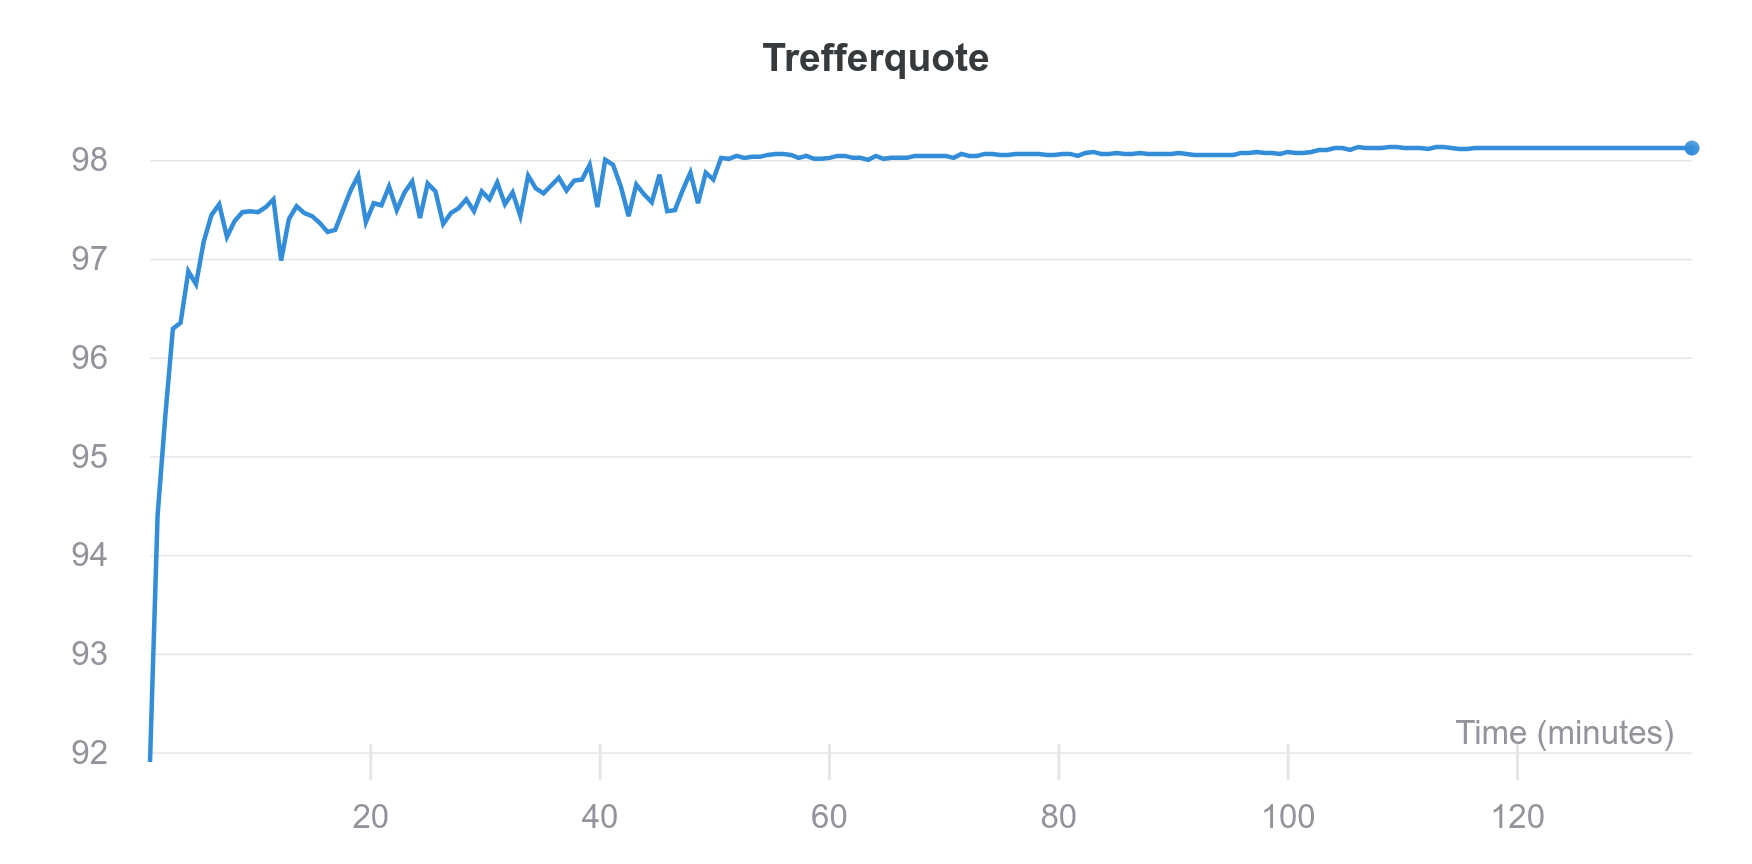
\includegraphics[width=0.9\linewidth]{../graphics/Wandb_accuracy.png}
	\caption{Ein Plot der Trefferquote, aufgetragen gegen die Trainingszeit}
	\label{accuracy}
\end{figure}
Aus den Daten geht hervor, dass der Anstieg der Trefferquote in den ersten 10 Epochen extrem groß ist. In den nächsten rund 65 Epochen schwankt sie zwischen etwa 97\% und 98\% und stagniert danach knapp über 98\%, wo sie nur noch eine geringe Steigung aufweist. Das Netz hat also nach 75 Epochen seinen Höhepunkt erreicht und konnte sich nicht weiter verbessern.\\
Dies korrespondiert auch mit dem in Abbildung \ref{loss} dargestellten Plot, der die Entwicklung des Kreuzentropiefehlers im Laufe des Trainings darstellt.
\begin{figure}[h]
	\begin{center}
	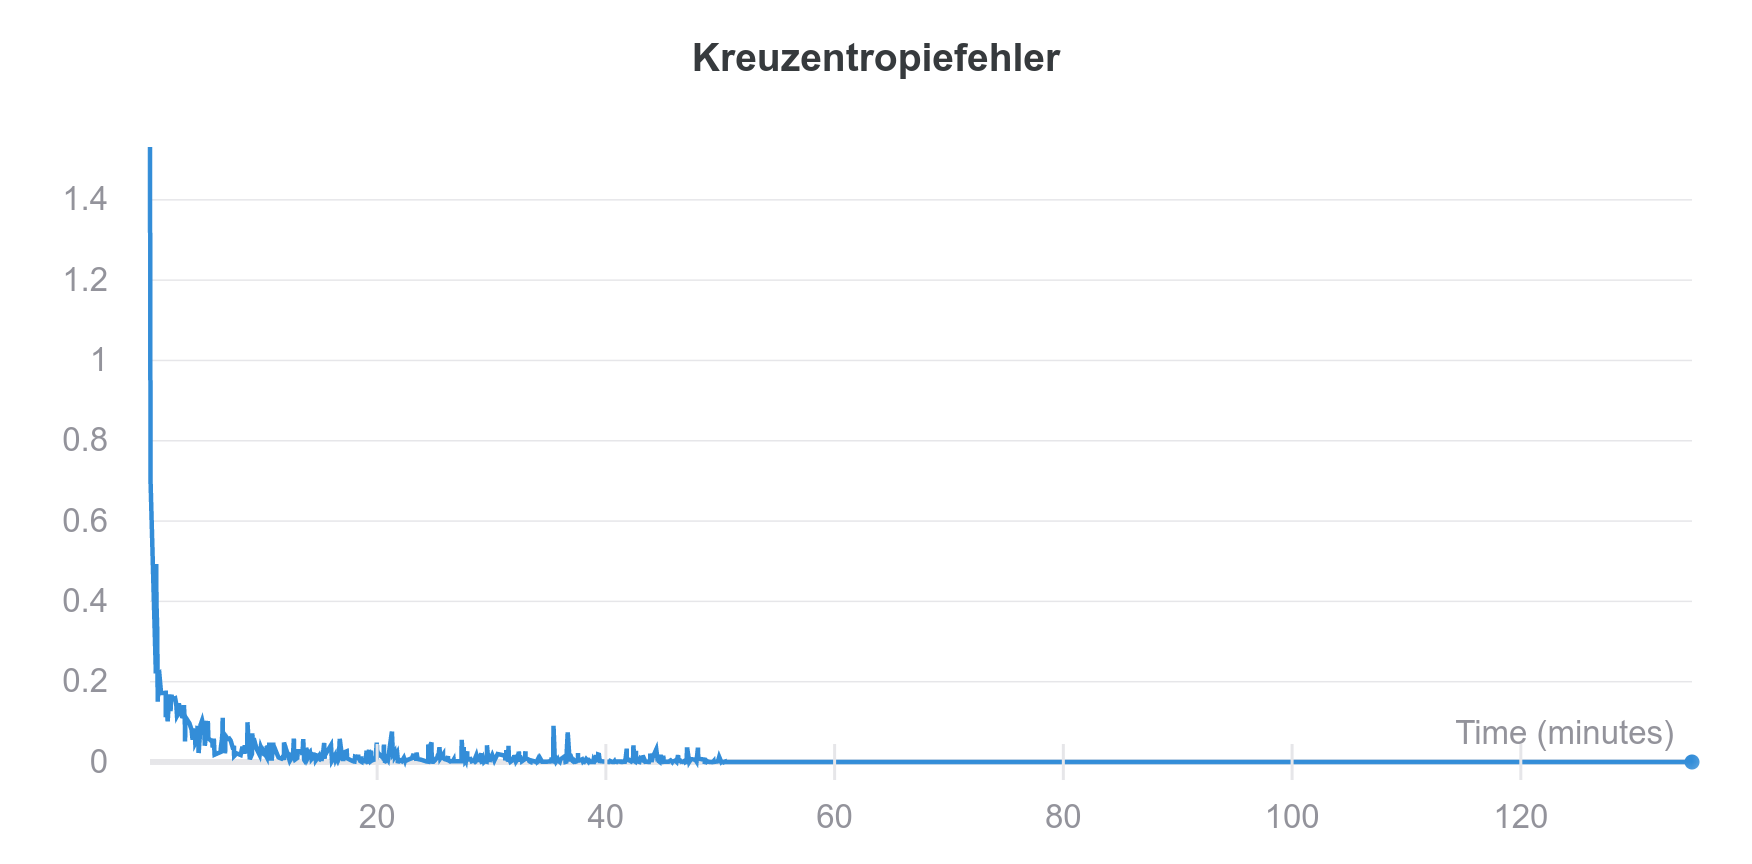
\includegraphics[width=0.9\linewidth]{../graphics/Wandb_loss.png}
	\end{center}
	\caption{Ein Plot des Kreuzentropiefehlers aufgetragen gegen die Trainingszeit}
	\label{loss}
\end{figure}
\\
Auch hier lässt sich ein extremes Abnehmen des Fehlers in den ersten 10 Epochen ablesen, das von einem starken Schwanken bis etwa zur 75. Epoche gefolgt ist. Von da an stagniert der Fehler bei 0. Das Ziel von 97\% Genauigkeit wurde also um einen Prozentpunkt überschritten, und somit lässt sich feststellen, dass das Netz sehr gut in der Lage ist, handgeschriebene Ziffern zu klassifizieren.
\section{Schluss}
Maschinelles Lernen ist ein extrem komplexes Forschungsgebiet, das ein enormes Potential aufweist. Die daraus hervorgehenden Technologien können auch das Alltagsleben revolutionieren und haben dies bereits in vielen Bereichen auch schon getan. Neuronale Netze stellen hier eine häufig verwendete Methode maschinellen Lernens dar. Sie sind an das menschliche Lernen angelehnt und können Klassifizierungs, Regressions und viele weitere Probleme lösen. Ihnen liegen algebraische Prozesse zugrunde, die häufig aus dem Bereich der Statistik stammen. Um die Netze zu trainieren, müssen große Datensätze vorhanden sein. Dies kann ein großes datenschutzrechtliches Problem darstellen. Die Ausgabe neuronaler Netze ist außerdem nie zu 100\% verlässlich. Trotz des großen Potentiales ist maschinelles Lernen jedoch nicht das Allheilmittel. Es kann zwar viele, aber bei weitem nicht alle Probleme lösen, und ist bei einem Großteil der  Probleme schlichtweg noch nicht effizient und verlässlich genug. Maschinelles Lernen hat dennoch Einzug in unser Alltagsleben gefunden, und wir begegnen ihm am Flughafen, im Supermarkt und am Smartphone (die Gesichtserkennungssoftware zum Entsperren vieler Geräte nutzt maschinelles Lernen, um eine höhere Genauigkeit zu erzielen). Von einer Welt, die von eigenständig handelnden und intelligenten Maschinen beherrscht wird, sind wir allerdings noch weit entfernt.\\
Es wurde auch gezeigt, dass Maschinelles Lernen durch Neuronale Netze eine Technik ist, die bereits mit geringem Aufwand in bekannten Programmiersprachen umgesetzt werden kann. Dabei ist es möglich durchaus gute Ergebnisse zu erzielen. Dafür können Frameworks wie PyTorch oder Tensorflow verwendet werden.
\newpage
\begin{thebibliography}{99}
	\bibitem{1}
	Hands-On Machine Learning with Scikit-Learn and TensorFlow\newline
	von Aurélien Géron\newline
	Veröffentlicht: March 2017 O'Reilly Media, Inc\newline
	ISBN: 9781491962282
	\bibitem{2}
	Die Logistik des Lernens eine Studie der LMU München\newline
	Quelle: www.uni-muenchen.de/forschung/news/2013/\newline f-71-13\_kiebler\_nervenzellen.html --abgerufen am 16.11.2019
	\bibitem{3}
	Common Loss functions in machine learning\newline
	Von Ravindra Parmar\newline
	Veröffentlicht am 02.09.2018, abgerufen am 07.01.2020\newline
	Quelle: https://towardsdatascience.com/common-loss-functions-in-machine-learning-46af0ffc4d23 
	\bibitem{4}
	Facial Recognition Is Everywhere at China’s New Mega Airport\\
	Bloomberg, 11. Dezember 2019\\
	https://www.bloomberg.com/news/articles/2019-12-11/face-recognition-tech-is-everywhere-at-china-s-new-mega-airport\\
	Abgerufen am 23.01.2020
	\bibitem{5}
	A US government study confirms most face recognition systems are racist\\
	20.12.2019 MIT technology review\\
	https://www.technologyreview.com/f/614986/ai-face-recognition-racist-us-government-nist-study/\\
	Abgerufen am 23.01.2020
	\bibitem{6}
	Offizielle Dokumentation des PyTorch Frameworks\\
	https://pytorch.org/docs/stable/nn.functional.html\\
	Abgerufen am 30.01.2020
	\bibitem{7}
	Adam: A Method for Stochastic Optimization\\
	Diederik P. Kingma und Jimmy Ba\\
	arXiv:1412.6980 [cs.LG] (https://arxiv.org/abs/1412.6980)\\
	Abgerufen am 31.01.2020
	\bibitem{8}
	Is BERT Really Robust? A Strong Baseline for Natural Language Attack on Text Classification and Entailment\\
	Di Jin, Zhijing Jin, Joey Tianyi Zhou und Peter Szolovits\\
	arXiv:1907.11932 [cs.CL] (https://arxiv.org/abs/1907.11932)\\
	Abgerufen am 12.02.2020
	\bibitem{9}
	Natural Adversarial Examples\\
	Dan Hendrycks, Kevin Zhao, Steven Basart, Jacob Steinhardt und Dawn Song\\
	arXiv:1907.07174 [cs.LG] (https://arxiv.org/abs/1907.07174)\\
	Abgerufen am 12.02.2020
	
\end{thebibliography}
\listoffigures
\end{document}